\documentclass[12pt,]{book}
\usepackage{lmodern}
\usepackage{amssymb,amsmath}
\usepackage{ifxetex,ifluatex}
\usepackage{fixltx2e} % provides \textsubscript
\ifnum 0\ifxetex 1\fi\ifluatex 1\fi=0 % if pdftex
  \usepackage[T1]{fontenc}
  \usepackage[utf8]{inputenc}
\else % if luatex or xelatex
  \ifxetex
    \usepackage{mathspec}
  \else
    \usepackage{fontspec}
  \fi
  \defaultfontfeatures{Ligatures=TeX,Scale=MatchLowercase}
\fi
% use upquote if available, for straight quotes in verbatim environments
\IfFileExists{upquote.sty}{\usepackage{upquote}}{}
% use microtype if available
\IfFileExists{microtype.sty}{%
\usepackage{microtype}
\UseMicrotypeSet[protrusion]{basicmath} % disable protrusion for tt fonts
}{}
\usepackage[margin=1in]{geometry}
\usepackage{hyperref}
\hypersetup{unicode=true,
            pdftitle={Challenges and Tools in the Assessment and Management of Pacific Salmon Fisheries},
            pdfauthor={Ben Staton},
            pdfborder={0 0 0},
            breaklinks=true}
\urlstyle{same}  % don't use monospace font for urls
\usepackage{natbib}
\bibliographystyle{apalike}
\usepackage{longtable,booktabs}
\usepackage{graphicx,grffile}
\makeatletter
\def\maxwidth{\ifdim\Gin@nat@width>\linewidth\linewidth\else\Gin@nat@width\fi}
\def\maxheight{\ifdim\Gin@nat@height>\textheight\textheight\else\Gin@nat@height\fi}
\makeatother
% Scale images if necessary, so that they will not overflow the page
% margins by default, and it is still possible to overwrite the defaults
% using explicit options in \includegraphics[width, height, ...]{}
\setkeys{Gin}{width=\maxwidth,height=\maxheight,keepaspectratio}
\IfFileExists{parskip.sty}{%
\usepackage{parskip}
}{% else
\setlength{\parindent}{0pt}
\setlength{\parskip}{6pt plus 2pt minus 1pt}
}
\setlength{\emergencystretch}{3em}  % prevent overfull lines
\providecommand{\tightlist}{%
  \setlength{\itemsep}{0pt}\setlength{\parskip}{0pt}}
\setcounter{secnumdepth}{5}
% Redefines (sub)paragraphs to behave more like sections
\ifx\paragraph\undefined\else
\let\oldparagraph\paragraph
\renewcommand{\paragraph}[1]{\oldparagraph{#1}\mbox{}}
\fi
\ifx\subparagraph\undefined\else
\let\oldsubparagraph\subparagraph
\renewcommand{\subparagraph}[1]{\oldsubparagraph{#1}\mbox{}}
\fi

%%% Use protect on footnotes to avoid problems with footnotes in titles
\let\rmarkdownfootnote\footnote%
\def\footnote{\protect\rmarkdownfootnote}

%%% Change title format to be more compact
\usepackage{titling}

% Create subtitle command for use in maketitle
\newcommand{\subtitle}[1]{
  \posttitle{
    \begin{center}\large#1\end{center}
    }
}

\setlength{\droptitle}{-2em}

  \title{Challenges and Tools in the Assessment and Management of Pacific Salmon
Fisheries}
    \pretitle{\vspace{\droptitle}\centering\huge}
  \posttitle{\par}
    \author{Ben Staton}
    \preauthor{\centering\large\emph}
  \postauthor{\par}
    \date{}
    \predate{}\postdate{}
  
\usepackage{booktabs}
%%% This is an example file for the Auburn University style options
%%%       aums.sty (Masters Thesis)
%%%       auphd.sty (Ph.D. Dissertation)
%%%       auhonors.sty (Honors Scholar)

%%%To use it, please edit the necessary options, title, author, date, year, keywords, advisor, professor, etc. 

% \documentclass[12pt]{report}
\usepackage{setspace}
% \usepackage{titlesec}
%\setcounter{secnumdepth}{3}
% \usepackage{aums}       % For Master's papers
\usepackage{auphd}     % For Ph.D.
%\usepackage{auhonors}  % For honors college
\usepackage[normalem]{ulem}       % underlining on style-page; see \normalem below
\usepackage{url}
\usepackage[table]{xcolor}
\usepackage{tikz}
\usepackage{pgf}
\usepackage{color,soul}
\usepackage{float}
\usepackage{caption}
\captionsetup{width=\textwidth}

\usepackage{amsmath,amsthm, amsfonts, mathrsfs, graphicx, setspace, fullpage, color}
\usepackage{natbib, appendix}
\usepackage[T1]{fontenc}
\usepackage{multirow}
\usepackage{mathabx}
\RequirePackage{adjustbox}
% \usepackage{epstopdf}
\AtBeginDocument{\renewcommand{\bibname}{References}}
\usepackage{hyperref}
%\usepackage{tocloft}
%\renewcommand\cftchapafterpnum{\vskip\baselineskip}
%\renewcommand\cftsecafterpnum{\vskip\baselineskip}
%\renewcommand\cftsubsecafterpnum{\vskip\baselineskip}
%\renewcommand\cftsubsubsecafterpnum{\vskip\baselineskip}
%\renewcommand\cftfigafterpnum{\vskip\baselineskip}
%\renewcommand\cfttabafterpnum{\vskip\baselineskip}

% remove double spacing from itemized lists
\usepackage{enumitem}
% \setlist[itemize]{noitemsep}
\setlist{before=\doublespacing,after=\doublespacing}


%%%%%Format rules: Normal margins are 1 in. If you need to print with 1.5in margins, uncomment the line below
%\oddsidemargin0.5in \textwidth6in

%% If you do not need a List of Abbreviations, then comment out the lines below and the \printnomenclature line.
%%for List of Abbreviations information:  (see http://www.mackichan.com/TECHTALK/509.htm  )
% \usepackage[intoc]{nomencl}
% \renewcommand{\nomname}{List of Abbreviations}   	       
% \makenomenclature 
%% don't forget to run:   makeindex ausample.nlo -s nomencl.ist -o ausample.nls
%% Also, if 

\makeatother
\let\oldmaketitle\maketitle
\AtBeginDocument{\let\maketitle\relax}

% Put the title, author, and date in. 
\title{Challenges and Tools in the Assessment and Management of Pacific Salmon Fisheries}
\author{Benjamin A. Staton} 
\date{May 5, 2019} %date of graduation
\copyrightyear{2019} %copyright year

\keywords{Fisheries management, Bayesian inference, decision analysis}

% Put the Thesis Adviser here. 
\adviser{Matthew J. Catalano}

% Put the committee here (including the adviser), one \professor for each. 
% The advisor must be first, and the dean of the graduate school must be last.
\professor{Matthew J. Catalano, AFFILIATION}

\professor{Asheber Abebe, AFFILIATION}

\professor{Lewis G. Coggins, Jr., AFFILIATION}

\professor{Conor P. McGowan, AFFILIATION}
\usepackage{booktabs}
\usepackage{longtable}
\usepackage{array}
\usepackage{multirow}
\usepackage[table]{xcolor}
\usepackage{wrapfig}
\usepackage{float}
\usepackage{colortbl}
\usepackage{pdflscape}
\usepackage{tabu}
\usepackage{threeparttable}
\usepackage{threeparttablex}
\usepackage[normalem]{ulem}
\usepackage{makecell}

\usepackage{amsthm}
\newtheorem{theorem}{Theorem}[chapter]
\newtheorem{lemma}{Lemma}[chapter]
\theoremstyle{definition}
\newtheorem{definition}{Definition}[chapter]
\newtheorem{corollary}{Corollary}[chapter]
\newtheorem{proposition}{Proposition}[chapter]
\theoremstyle{definition}
\newtheorem{example}{Example}[chapter]
\theoremstyle{definition}
\newtheorem{exercise}{Exercise}[chapter]
\theoremstyle{remark}
\newtheorem*{remark}{Remark}
\newtheorem*{solution}{Solution}
\begin{document}
\maketitle

\begin{romanpages}      % roman-numbered pages 

\TitlePage 

\doublespacing
\setlength{\parskip}{0pt plus 0pt minus 0pt}

\begin{abstract} 
\noindent
I'm going to write an abstract to go here. This is the first paragraph of the dissertation abstract, which will talk about chapter 1..

This is the second paragraph of the dissertation abstract, which will talk broadly about chapter 2.

This is the third paragraph of the dissertation abstract, which will talk broadly about chapter 3.

This is the fourth paragraph of the dissertation abstract, which will talk broadly about chapter 4.
\end{abstract}

\begin{acknowledgments}
\noindent
Here is where I will thank everyone.

Matt, Lew, Brendan, Mike, Sam, AL-HPC folks, Steve, Nick, Zach, Janessa. Family and Michelle. Folks at the lab. RStudio staff.
\end{acknowledgments}

\begin{singlespace}
	\tableofcontents
	\clearpage
	\listoffigures
	\clearpage
	\listoftables
\end{singlespace}

% \printnomenclature[0.5in] %used for the List of Abbreviations
\end{romanpages}        % All done with roman-numbered pages

\normalem       % Make italics the default for \em

% \titlespacing\section{0pt}{12pt plus 4pt minus 2pt}{0pt plus 2pt minus 2pt}
% \titlespacing\subsection{0pt}{12pt plus 4pt minus 2pt}{0pt plus 2pt minus 2pt}
% \titlespacing\subsubsection{0pt}{12pt plus 4pt minus 2pt}{0pt plus 2pt minus 2pt}

\setlength{\parskip}{0pt plus 0pt minus 0pt}

\doublespacing

\chapter*{Preface}\label{preface}
\addcontentsline{toc}{chapter}{Preface}

I used bookdown \citep{xie-2015} to make this document.

\chapter{Development and Evaluation of a Migration Timing Forecast Model
for Kuskokwim River Chinook Salmon}\label{ch2}

\section*{Abstract}\label{abstract}
\addcontentsline{toc}{section}{Abstract}

Annual variation in adult salmon migration timing makes the
interpretation of in-season assessment data difficult, leading to much
in-season uncertainty in run size. We developed and evaluated a run
timing forecast model for the Kuskokwim River Chinook salmon stock,
located in western Alaska, intended to aid in reducing this source of
uncertainty. An objective and adaptive approach (using model-averaging
and a sliding window algorithm to select predictive time periods, both
calibrated annually) was adopted to deal with multidimensional selection
of four climatic variables and was based entirely on predictive
performance. Forecast cross-validation was used to evaluate the
performance of three forecasting approaches: the null (i.e., intercept
only) model, the single model with the lowest mean absolute error, and a
model-averaged forecast across 16 nested linear models. As of 2018, the
null model had the lowest mean absolute error (2.7 days), although the
model-averaged forecast performed as well or better than the null model
in the majority of retrospective years and currently has a mean absolute
error of 3.2 days. The model-averaged forecast had a consistent mean
absolute error regardless of the type of year (i.e., average or extreme
early/late) the forecast was made for, which was not true of the null
model. The availability of the run timing forecast was not found to
increase overall accuracy of in-season run assessments in relation to
the null model, but was found to substantially increase the precision of
these assessments, particularly early in the season.

\section{Introduction}\label{introduction}

\noindent
In-season management strategies for Pacific salmon (\emph{Oncorhynchus}
spp.) fisheries rely heavily on indices of in-river abundance (e.g.,
test fisheries, sonar counts, etc.) to inform harvest control rules that
attempt to attain the balance of meeting pre-determined escapement
objectives while allowing adequate opportunity for harvest
\citep{catalano-jones-2014}. However, because indices of abundance are
confounded by the phenology (i.e., timing) of the migration, their
interpretation is very difficult in-season. For example,
smaller-than-average index values early in the season could be due to
either a small run with average timing or by a late large run, when
interpreted in the context of historical years
\citep{adkison-cunningham-2015}. This ultimately leads to great
uncertainty about how much of the incoming run has passed, which is a
key piece of information that dictates fishery harvest opportunities.
There exists no information in the current year's abundance index to
inform the manager if (for example) 25\% or 75\% of the run has passed
on any given day. Yet, depending which is true, the optimal management
decision could be vastly different. Thus, in-season assessment typically
involves some characterization of the variation in historical run timing
to formulate a range of possible run size scenarios that could be
representative of the current year's run size. However, given the amount
of variation in historical run timing, these scenarios are rarely
informative during the majority of the migration, when key harvest
decisions are being made because the run scenarios may span all possible
run sizes. As a result, the pre-season run size forecast remains the
most precise piece of information for much of the season. If it were
possible to predict the timing of the incoming run (e.g., earlier- or
later-than-average) with some level of confidence, it could prove
valuable for in-season assessment and decision-making by reducing
uncertainty in run size predictions.

While previous research has uncovered several key physiological
mechanisms that are involved with natal homing
\citep{hasler-scholz-1983} and return migrations of adult salmon to
freshwater environments
\citep{cooperman-etal-2010, cooke-etal-2008, hinch-etal-2012}, the exact
physiological and behavioral responses of adult salmon to relatively
small-scale environmental gradients within estuaries, which are likely
the ultimate determinants of freshwater entry timing, are still poorly
understood. Despite this uncertainty, several hypotheses have been put
forth that are broadly consistent with the observed timing patterns of
several species across a large geographic area (i.e., western and
southwestern Alaska). Two primary influences have been suggested:
genetic \citep{quinn-etal-2000, anderson-beer-2009, omalley-etal-2010}
and environmental \citep{hodgson-etal-2006, keefer-etal-2008}
mechanisms. Substantial evidence exists to suggest that both genetic and
environmental controls are involved in determining migration timing,
however it is broadly thought that genetic variation influences
sub-stock variation (i.e., different tributary spawning groups within
the same major river basin) and environmental variation influences the
timing of the aggregate (i.e., basin-wide) run
\citep{keefer-etal-2008, anderson-beer-2009}. This is consistent with
the notion that genetically distinct components of the aggregate run
behave differently as a result of their life history strategies and/or
the characteristics of their specific spawning grounds
\citetext{\citealp[e.g., sub-stocks that must travel farther in-river to
reach spawning grounds enter freshwater
earlier;][]{clark-etal-2015}; \citealp[sub-stocks that spawn in
tributaries influenced by warmer lakes enable later
spawning;][]{burger-etal-1985}} but that certain environmental
conditions act on the aggregate run to either hasten or delay freshwater
entry. It has also been suggested that run size may have an influence on
migration timing, although empirical support for this claim seems to be
lacking. If there were indeed relationships between run timing and run
size, these need to be quantified as certain combinations are
particularly troublesome for managers \citep[e.g., small/early runs and
large/late runs appear the same early
in-season;][]{adkison-cunningham-2015}.

At the aggregate population scale, which is the focus of this Chapter,
it has been observed that migrations occurring in the spring and summer
generally occur earlier in years with warmer spring temperatures
\citep{mundy-evenson-2011, hodgson-etal-2006}.
\citet{mundy-evenson-2011} suggested that this pattern may be explained
by the stability of the estuarine water column where adult salmon stage
in preparation for riverine entry (or alternatively, marine exit). High
estuarine water column stability was hypothesized to impede riverine
entry through two mechanisms:

\begin{enumerate}
\def\labelenumi{(\arabic{enumi})}
\tightlist
\item
  by presenting an osmotic barrier between freshwater riverine discharge
  and the saline ocean water which prevents osmotically incompetent
  individuals from crossing and,
\item
  by preventing freshwater competent individuals from receiving
  olfactory cues essential to the homeward migration.
\end{enumerate}

\noindent
Thus, \citet{mundy-evenson-2011} hypothesized that years in which the
estuarine water column is stable over a longer period of time would be
associated with later migration timing. Although water column stability
is a difficult variable to measure over large spatial scales, several
variables that are known to influence it are available at large scales
via remote sensing (e.g., satellite observations). Such variables are
sea ice cover which prevents wind-driven mixing, associated local
temperature-related variables like land-based air temperature or sea
surface temperature (SST), and broader scale indicators such as the
Pacific Decadal Oscillation (PDO), an index of temperature anomalies in
the northern Pacific Ocean. Observational studies across the North
American range of Chinook salmon have found environmental-run timing
correlations that are consistent with this hypothesis
\citep{hodgson-etal-2006, keefer-etal-2008, mundy-evenson-2011}. Even if
the water column stability hypothesis is incorrect, observed patterns
suggest that environmental variables may be useful in forecasting run
timing with some level of accuracy and certainty.

Several efforts have been made at exploiting these environmental-run
timing relationships to develop run timing forecast models for Pacific
salmon migrations. \citet{mundy-evenson-2011} developed a model for
Yukon River Chinook salmon (\emph{O. tshawytscha}) that used air
temperature, SST, and ice cover to predict the day at which the
\(15^{\text{th}}\) and \(50^{\text{th}}\) percentiles of the run passed
a test fishery index location. Their model predictions fit the observed
data well (nearly always within seven days, usually within three days),
although out-of-sample predictive ability was not presented.
\citet{keefer-etal-2008} developed a similar framework for Columbia
River spring run Chinook salmon and found run timing relationships with
river discharge, river temperature, and ocean condition indices (e.g.,
PDO). Their best model explained 49\% of the variation in median run
timing with variation in the environmental variables.
\citet{anderson-beer-2009} continued this work on the Columbia River
spring Chinook stock, but added genetic components to their analysis
based on the arrival timing of precocious males. Their findings revealed
that both environmental variables and changes in abundance of
genetically distinct populations, which had their own distinct migration
timing and affected overall run timing of the spring Chinook salmon run
in the Columbia River. These advancements have shown that relationships
between migration timing and environmental variables exist and may have
utility for use in forecasting efforts.

The Kuskokwim River, located in western Alaska, is the second largest
river system in the state and supports culturally and economically
important Chinook salmon fisheries. Chinook salmon return beginning in
late May and continue through early August, with the median date of
passage occurring between June 14 and July 2. Fisheries within the
region harvest salmon in-river during freshwater migrations using
primarily drift gillnet gear. The Kuskokwim River salmon fishery has a
distinct cultural importance: nearly all inhabitants are native Alaskans
belonging to the Yup'ik group and take salmon for subsistence purposes
\citep{linderman-bergstrom-2009}. While commercial salmon fisheries
operate within the river, these fishers often also participate in
subsistence take and revenues from the sale of commercially-harvested
salmon often contribute directly to participation in subsistence
activities \citep{wolfe-spaeder-2009}. To ensure long-term sustainable
harvest, the Chinook salmon fishery is managed with a drainage-wide
escapement goal derived from an age-structured state-space
spawner-recruit analysis \citep{hamazaki-etal-2012, staton-etal-2017a}.
To meet these pre-determined escapement goals, in-season management
strategies implement time, gear, and area closures based on limited and
imprecise information regarding annual run size. The distant locations
of the majority of escapement assessment projects makes direct
measurement of escapement performance unavailable until late in the
season. Thus, the primary sources of run size assessment information are
(1) a pre-season run size forecast range (obtained as the previous
year's run size estimate \(\pm \sim 20\%\)) and (2) an in-river drift
gillnet test fishery operated in Bethel, AK which has been implemented
using consistent methods since 1984. The interpretation of this test
fishery index suffers from the same issue of being confounded by run
timing described earlier, making management decisions difficult. Without
precise in-season indicators of run size, managers must often choose to
either trust a pre-season run size forecast for the majority of the
season or somehow place weights on the various run timing hypotheses
when interpreting in-season data. Both options could lead to the wrong
interpretation of the actual run size, which could have serious
consequences for the management of the fishery in a given year (i.e.,
the unwarranted opening or closing the fishery resulting in severe
under- or over-escapement). No published run timing forecast models
currently exist for Kuskokwim River Chinook salmon but given the
potential utility of independent run timing estimates for interpretation
of in-season data, the development and evaluation of such a model is
needed. The necessity of more accurate and precise in-season perceptions
of run size is particularly evident in years with anticipated low runs,
such as in recent years (i.e., since 2010), as this may allow managers
to more effectively guard against over-exploitation while still allowing
for limited harvest opportunities to support the cultural and
subsistence needs of the region.

In this chapter, I present an analysis that develops and evaluates the
performance of a run timing forecast model for Kuskokwim River Chinook
salmon. The objectives were to

\begin{enumerate}
\def\labelenumi{(\arabic{enumi})}
\tightlist
\item
  quantify historical run timing,
\item
  develop a run timing forecast model using environmental variables
  selected based on out-of-sample predictive performance
\item
  assess the utility of the forecasting model for improving predictions
  of end-of-season test fishery indices of run size,
\item
  determine if there is a relationship between run size and run timing
  for the Kuskokwim River Chinook salmon stock.
\end{enumerate}

\section{Methods}\label{methods}

\subsection{Estimates of migration
timing}\label{estimates-of-migration-timing}

\noindent
In this analysis, the forecasted quantity that represented migration
timing was the day at which 50\% of the run passed an index location
(hereafter, \(D_{50}\)). To inform this quantity for each year in the
analysis, we used daily catch-per-unit-effort (CPUE) data from the
Bethel Test Fishery (BTF) operated by the Alaska Department of Fish and
Game (ADF\&G), which spans 1984 -- 2018. The raw data were daily CPUE
beginning on June 1 and ending August 24 each year. The cumulative sum
of these daily CPUE values within a year follows a sigmoidal pattern
reflecting the shape of the incoming salmon run which is characterized
by relatively few early migrants, a peak where the majority of the fish
are running, and relatively few late migrants. To estimate the median
day of passage as a continuous variable, a logistic model was fitted to
the cumulative proportion of daily CPUE of the form:

\begin{equation}
  p_{d,t}=\frac{1}{1 + e^{-h_t (d - D_{50,t})}},
  \label{eq:logistic}
\end{equation}

\noindent
where \(p_{d,t}\) is the predicted cumulative proportion on
day-of-the-year (DOY) \(d\) in calendar year \(t\), \(h_t\) is the
parameter that controls the steepness of the curve (i.e., duration of
the run), and \(D_{50,t}\) is the day at which 50\% of the total annual
CPUE was caught in year \(t\). Annual estimates of \(D_{50,t}\) and
\(h_t\) were obtained by fitting \(p_{d,t}\) to observed daily
cumulative proportion by minimizing the sum of squared deviations from
the model prediction. Uncertainty in these parameter estimates was not
considered further in the analysis as the uncertainty was negligible.
Further, the use of the BTF daily CPUE values to infer the location and
shape of year-specific logistic timing curves made the assumption that
these data provided an accurate representation of daily run strength
within a year (i.e., that the influence of weather conditions or harvest
on sampling was negligible).

\subsection{Environmental variables}\label{environmental-variables}

\noindent
Environmental variables to be assessed for forecasting performance were
chosen based on three criteria:

\begin{enumerate}
\def\labelenumi{(\arabic{enumi})}
\tightlist
\item
  previously established association with salmon run timing,
\item
  availability for the Kuskokwim River during the years for which BTF
  index observations exist (1984 -- 2018), and
\item
  availability for use in a pre-season forecast model (i.e., available
  no later than June 10\textsuperscript{th} in the year for which the
  forecasted value would be used).
\end{enumerate}

\noindent
Based on these criteria, four environmental variables were chosen for
analysis: SST, percent sea ice cover (SIC), PDO, and land-based air
temperature taken in Bethel, AK.

\subsubsection{PDO data}\label{pdo-data}

\noindent
Data collected for the PDO variable came from one of several indices
produced by the National Oceanic and Atmospheric Administration (NOAA)
\citep{mantua-etal-1997}\footnote{PDO data:
  \url{http://research.jisao.washington.edu/pdo/PDO.latest.txt}}. The
index is produced by taking the first principal component of monthly SST
anomalies in the northern Pacific Ocean, after removing any global
trends due to any systematic change over time \citep{mantua-etal-1997}.
Thus, for each year of the data set, a single monthly value was
available for PDO. Previous studies have found PDO values prior to the
initiation of the run have predictive value for Chinook salmon
populations \citep{beer-2007, keefer-etal-2008}.

\subsubsection{Bethel air temperature
data}\label{bethel-air-temperature-data}

\noindent
Air temperature data for Bethel, AK were accessed from the Alaska
Climate Research Center\footnote{Alaska air temperature data:
  \url{http://akclimate.org/acis_data}}. These data were available as
daily means for each day of each year in the 1984 -- 2018 data set.

\subsubsection{SST and SIC}\label{sst-and-sic}

\noindent
SST and SIC data were accessed from the NOAA Optimum Interpolation SST
V2 High Resolution Dataset \citep{reynolds-etal-2007}\footnote{Global
  gridded SST and SIC:
  \url{http://www.esrl.noaa.gov/psd/data/gridded/data.noaa.oisst.v2.highres.html}}.
These data were available as daily means for any 0.25° by 0.25° latitude
by longitude grid cell on the globe. To limit the search, only grid
cells within Kuskokwim Bay were selected for analysis Figure
\ref{fig:ch2-map} as that is the area that Chinook salmon bound for the
Kuskokwim River likely aggregate prior to riverine entry. The area with
grid cells ranged from 58.5° N to 60° N by 164.25° W to 162° W, which
resulted in a total of 54 0.25° latitude by 0.25° longitude grid cells.
For SST, four grid cells fell partially over land (resulting in 50 grid
cells with daily data) and for SIC, five grid cells were partially over
land (49 grid cells with daily data). ``Empty'' grid cells were excluded
and the remaining grid cells were used for prediction. Previous analyses
have used a simple average over a wide spatial area
\citep[e.g.,][]{mundy-evenson-2011} to create a single value for SST or
SIC each year. However, this is somewhat arbitrary and does not account
for the possibility of certain areas having stronger timing signals than
others or that the areas with stronger signals may change over time.
Thus, the gridded spatial structure of these variables was retained and
the treatment of this structure in the forecast analysis is discussed
below in Section \ref{rtf-models}.

\subsection{Forecast model}\label{reg-models}

To produce a forecast of run timing, relationships between historical
observed pairs of the environmental variables each year and \(D_{50,t}\)
must be quantified. The simple linear regression framework was used to
obtain these historical relationships:

\begin{equation}
  \begin{split}
    D_{50,t} = \beta_0 + \beta_j x_{t,j} +,...,+ \beta_n x_{t,J} + \varepsilon_t, \\
    \varepsilon_t \stackrel{\text{iid}}{\sim} N(0, \sigma) \\
  \end{split}
\label{eq:lin-reg}
\end{equation}

\noindent
where \(D_{50,t}\) is the observed run timing value in year \(t\),
\(x_{t,j}\) is the observed value of covariate \(j\) (of which there are
\(J\) included in the model), \(\beta_0\) and \(\beta_j\) are
coefficients linking the observed values of \(D_{50,t}\) with
\(x_{t,j}\), \(\varepsilon_t\) are random residual effects that explain
deviations of observed \(D_{50,t}\) from the fitted value and have
constant variance equal to \(\sigma^2\).

There are many such regression models that could be used to produce a
run timing forecast (i.e., \(\hat{D}_{50,t+1}\)). This is because:

\begin{enumerate}
\def\labelenumi{(\arabic{enumi})}
\tightlist
\item
  there are four variables (PDO, air temperature, SST, and SIC) that
  could be included,
\item
  each variable is temporally structured, i.e., there are daily or
  monthly values for each variable, and
\item
  two variables (SST and SIC) are spatially-explicit, i.e., there are
  different values for each day and year for different areas of
  Kuskokwim Bay (Figure \ref{fig:ch2-map}).
\end{enumerate}

\noindent
Item (1) deals with the specific values of \(j\) and \(J\) whereas items
(2) and (3) deal with what values of \(x_{t}\) for a given \(j\) should
take on.

\subsection{Selection of predictive time periods}\label{clim-windows}

\noindent
To fit the regression model in Equation \eqref{eq:lin-reg}, a single value
for each \(x_{t,j}\) was required. The covariate data were temporally
structured, however, indicating that some selection of which time
periods to use to populate \(x_{t,j}\) was needed. Oftentimes the
average over an arbitrary time period, such as daily values in the month
of February, is used based on \emph{a priori} assumptions of the
behavior of important factors \citep{vandepol-etal-2016}. While this
approach is simple to implement and explain, it is possible that a
better time window (i.e., reliably more accurate) exists but was not
considered. Furthermore, the importance of various time windows may
change over time and the arbitrary selection of a single window does not
allow for such changes to be detected. To avoid these issues, a rigorous
temporal selection process, known as the sliding climate window
algorithm \citep[SCWA;][]{vandepol-etal-2016}, was implemented to
determine the best predictive time period for each variable considered
in the forecast model. To find the most reliable temporal window for
prediction, the SCWA evaluates all possible windows (subject to certain
restrictions) over which to average for use as the predictor variable in
the forecast model. The following section provides the details of the
SCWA.

\subsubsection{The SCWA}\label{the-scwa}

\noindent
A ``window'' in this context is hereafter defined as a block of
consecutive days in some portion of the year with starting
day-of-the-year (DOY) denoted by \(D_F\) and ending day equal to
\(D_L\). The daily values within each evaluated window were averaged for
the \(x_{t,j}\) value to be used in a linear regression framework. As
input constraints, the SCWA used in this analysis required:

\begin{enumerate}
\def\labelenumi{(\arabic{enumi})}
\tightlist
\item
  the start date of the first window to be evaluated (\(D_0\)),
\item
  the end date of the last window to be evaluated (\(D_n\)), and
\item
  the minimum window size of a candidate window (\(\Delta_{D,min}\)).
\end{enumerate}

\noindent
The algorithm started with the earliest and smallest possible time
window: \(D_F = D_0 = 1\) through
\(D_L = D_0 + \Delta_{D,min} - 1 = 5\). The performance of this window
when used to obtain \(x_{t,j}\) was evaluated (see Section \ref{fcst-cv}
below) and the result was stored for comparison to other candidate
windows. For the next window, \(D_F\) would remain at \(D_0\), but
\(D_L\) would be incremented by 1 day (\(\ell=1\)). Thus, the endpoints
of all candidate windows with \(D_F = D_0\) can be generalized as:

\begin{equation}
  [D_0, D_0 + \Delta_{D,min} - 1 + \ell],
\label{eq:scwa-1}
\end{equation}

\noindent
for each \(\ell = 0, 1, ..., n - 1\), where \(n = D_L - D_F + 1\). For
all windows, including those with \(D_F = D_0\), this generalizes to:

\begin{equation}
  [D_0 + f, D_0 + f + \Delta_{D,min} - 1 + \ell],
\label{eq:scwa-2}
\end{equation}

\noindent
for each \(f = 0, 1, ..., n - \Delta_{D,min}\) and
\(\ell = 0, 1, ..., n - \Delta_{D,min} - f\). Windows with
\(f > n - \Delta_{D,min}\) would contain fewer than \(\Delta_{D,min}\)
days and are thus prohibited. After evaluating all windows, the single
window with the best predictive performance was used to obtain the
forecast predictor variable for that data source (i.e., PDO
\emph{versus} air temperature). As an example, consider the following
inputs:

\begin{itemize}
\tightlist
\item
  \(D_0 = 1\) (i.e., the first day of the year),
\item
  \(D_n = 31\) (i.e., January 31), and
\item
  \(\Delta_{D,min}\) = 5.
\end{itemize}

The SCWA would start with January 1 -- January 5, then do January 1 --
6, January 1 -- 7, etc., January 1 -- 31. Next, it would exclude January
1 from consideration and evaluate all windows starting with January 2.
When it completes the one window starting with January 27, it must stop
because windows starting later than January 27 would result in windows
shorter than 5 days.

The values of \(D_0\) and \(D_L\) for the four covariates are shown in
Table \ref{tab:scwa-dates-table}. The setting for \(\Delta_{D,min}\) for
air temperature, SST, and SIC was set to 5 days. Note that because PDO
was available in monthly values only, each month was treated as ``day''
in the algorithm described above and \(\Delta_{D,min}\) was set to 1.

\subsubsection{Forecast cross-validation}\label{fcst-cv}

A metric was needed to measure the performance of the many windows. This
metric was obtained using a time series forecast cross-validation
procedure, which is an out-of-sample technique for data that are
collected through time \citep{arlot-celisse-2010}. The procedure
operated by producing a forecasted value of \(D_{50}\) for year \(t+1\)
trained based on all data \(x_{t,j}\) available from years
\(1, ..., t\). It then continued for all \(t = m, ..., n-1\), where
\(m\) is the minimum number of years necessary to fit the model (set at
\(m = 10\) in all cases) and \(n\) is the number of years of available
data. Then, absolute forecast error in was calculated based on all
forecasted years as \(|D_{50,t+1} - \hat{D}_{50,t+1}|\), and yearly
forecast errors were averaged to obtain mean absolute error
(\(\overline{\text{AE}}\)) which was used as the measure of model
performance in window selection. The window with the lowest
(\(\overline{\text{AE}}\)) was selected as the optimal window to average
over for prediction. The forecasting cross-validation procedure was used
as opposed to other out-of-sample validation procedures, such as
\(k\)-fold or leave-one-out methods, because the data were collected
through time and the forecast model would never need to predict (for
example) year 2010 from years 1984 -- 2009 and 2011 -- 2018, but rather
it would always need to predict year \(t+1\) from all
previously-collected data.

When forecasting \(D_{50,t+1}\) from training data from \(1,...,t\), a
single optimal climate window was selected for each variable and that
window was used to estimate coefficients based on training data and
obtain the environmental variable value for prediction in year \(t+1\)
to forecast \(D_{50,t+1}\). When a new year of data was added to the
training data (such as in the retrospective forecast analysis; Section
\ref{retro}), the optimal window for each variable was re-assessed using
the algorithm again. For PDO and Bethel air temperature, which had no
spatial structure, the SCWA was used to select the range of monthly
(PDO) or daily (Bethel air temperature) values to include in the
predictive climate window for each year in the analysis. For SST and SIC
which contained a series of 50 and 49 grid cells, respectively, each
with unique daily values, the SCWA was used on each grid cell
separately. The result was 50 unique grid cell-specific windows for SST
and 49 windows for SIC for each year of the analysis. The treatment of
this spatial structure in the forecast analysis is discussed below in
Section \ref{rtf-models}.

\subsection{Evaluated forecast models}\label{rtf-models}

\noindent
Linear regression \eqref{eq:lin-reg} was used to assess the forecast
performance of each of the variables described above, both in isolation
of and in combination with other variables. All possible subsets were
evaluated (excluding interactive effects) for predictive ability through
time, resulting in a total of 16 models ranging from the null (i.e.,
intercept only) model to the full (i.e., global) model (all four
variables as additive predictors).

For the spatially-explicit variables (i.e., SST and SIC), a more complex
treatment was required to prevent all grid cell values from being used
as predictors in a single model. To handle the spatial structure, grid
cell-specific regression models were fitted, then model-averaging based
on AIC was used to obtain a single forecast \(D_{50}\) for each year
\citep{burnham-anderson-2002}. Under this approach, each grid cell \(g\)
received an AIC\textsubscript{c} score:

\begin{equation}
  \text{AIC}_{c,g}=n \log{\left(\hat{\sigma}_g^2\right) + 2K + \frac{2K(K+1)}{n-K-1}},
  \label{eq:aicc}
\end{equation}

\noindent
where \(n\) is the number of data points used in each model,
\(\hat{\sigma}_g\) is the estimate of the residual standard deviation
under grid \(g\), and \(K\) is the number of model parameters. The
corrected version of AIC (AIC\textsubscript{c}) is recommended in cases
where the ratio of \(n\) to \(K\) is small (Burnham and Anderson, 2002).
Then, each grid cell received a \(\Delta\text{AIC}_\text{c}\) score,
representing its relative performance in comparison to the best grid
cell:

\begin{equation}
  \Delta_g=\text{AIC}_{\text{c},g}-\text{AIC}_{\text{c},min},
  \label{eq:delta-aicc}
\end{equation}

\noindent
where \(\text{AIC}_{\text{c},min}\) is the minimum AIC\textsubscript{c}
across all grid cells. Model (grid cell) weights were then calculated
as:

\begin{equation}
  w_g=\frac{e^{-0.5\Delta_g}}{\sum_j^G e^{-0.5\Delta_j}},
\label{eq:aicc-weights}
\end{equation}

\noindent
where \(G\) is the number of grid cells. Grid cell-averaged predictions
were then obtained as:

\begin{equation}
  \hat{y}_{t+1}=\sum_g^G w_g \hat{y}_{g,t+1},
\label{eq:grid-avg-fcst}
\end{equation}

\noindent
where \(\hat{y}_{g,t+1}\) is the forecasted value of \(D_{50}\) for grid
cell \(g\).

\subsection{Forecast uncertainty}\label{forecast-uncertainty}

\noindent
In addition to forecast accuracy, forecast precision is also of great
importance. For models that did not require AIC\textsubscript{c}
model-averaging across grid cells, the following equation was used to
produce a forecast standard error (SE):

\begin{equation}
  \text{SE}=\hat{\sigma} \sqrt{1 + \frac{1}{n} + \frac{(x-\bar{x})^2}{\sum_i^n(x_i-\bar{x})^2}},
\label{eq:se}
\end{equation}

\noindent
where \(n\) is the number of years the model was fitted to, \(x\) is the
value of the predictor variable used for forecasting, and \(\bar{x}\) is
the mean of all predictor values excluding the new value used for
forecasting. For models that used AIC\textsubscript{c} model-averaging
(i.e., those including SST and SIC), the following equation was used to
produce prediction SE:

\begin{equation}
  \text{SE}=\sum_g^G w_g \sqrt{\text{SE}_g^2+(\hat{y}_{g,t+1}-\hat{y}_{t+1})^2},
\label{eq:mod-avg-se}
\end{equation}

\noindent
where \(\text{SE}_g\) is the prediction SE from grid cell \(g\)
calculated using \eqref{eq:se}. This estimator of unconditional sampling
standard error accounts for uncertainty within each model and the
uncertainty due to model selection \citep{burnham-anderson-2002}.
Prediction intervals were calculated using the point estimate of
prediction, the prediction SE, and appropriate quantiles from the
corresponding \(t\)-distribution.

\subsection{Forecast model selection}\label{model-selection}

\noindent
Given 16 forecast models, it is impossible to know which will perform
the best at forecasting for the current year. Thus, three methods to
obtain a forecast for \(D_{50}\) were evaluated:

\begin{enumerate}
\def\labelenumi{(\arabic{enumi})}
\tightlist
\item
  the null (i.e., intercept only) model,
\item
  the single model with the lowest forecast cross-validation score as of
  the last year, and
\item
  model-averaging across the ensemble of 16 forecast models based on
  AIC\textsubscript{c} scores.
\end{enumerate}

\noindent
According to \citet{burnham-anderson-2002}, model-averaging should
perform better than a single ``best model'' at prediction when there is
a high degree of uncertainty about which model is best. This procedure
was performed using \eqref{eq:aicc} -- \eqref{eq:mod-avg-se}, by
substituting the prediction, prediction SE, and \(K\) for forecast model
\(i\), in place of grid \(g\). Prediction intervals based on
model-averaged predictions and prediction SE present somewhat of a
problem when the different models contributing to the average contain
differing degrees of freedom as it is unclear how many standard errors
the prediction limits should lie from the mean prediction. Thus, the
estimator suggested by \citet{burnham-anderson-2002} of the ``adjusted
SE'' (ASE) was used:

\begin{equation}
  ASE=\sum_i^{16} w_i \sqrt{\left(\frac{t_{df_i,1-\alpha/2}}{z_{1-\alpha/2}}\right)^2 \text{SE}_i^2+(\hat{y}_{i,t+1}-\hat{y}_{t+1})^2},
\label{eq:ase}
\end{equation}

\noindent
where \(t_{df,i,1-\alpha/2}\) is the \(1-\alpha/2\) quantile of the
\(t\) distribution with degrees of freedom equal to that of model \(i\)
and \(z_{1-\alpha/2}\) is the corresponding quantile of the \(z\) (i.e.,
standard normal) distribution. The confidence level \(\alpha = 0.05\)
was used in all cases.

\subsection{Retrospective forecast analysis}\label{retro}

\noindent
The analysis was conducted in a retrospective forecast framework
starting in 1994. All data after 1994 were ignored, optimal windows were
selected for each of the four variables (and all grids for SST and SIC),
all 16 models were fitted, a \(D_{50}\) forecast was made for 1995 using
the three approaches described in Section \ref{model-selection}, and
each was evaluated for predictive accuracy. This process was repeated
annually until the present (i.e., out-of-sample predictions made for
1995 -- 2018), which allowed for the calculation of
\(\overline{\text{AE}}\) through time as if the forecast model would
have been available beginning in spring 1995. In addition to
\(\overline{\text{AE}}\), median absolute error
\(\widetilde{\text{AE}}\)) was calculated to validate prediction
accuracy of estimates by ignoring the effect of outlying poor
predictions.

\subsection{Value of forecast to run size assessments}\label{eos-preds}

\noindent
It is important to remember that the purpose of producing a run timing
forecast is to aid in the interpretation of in-season indices of run
size such as test fisheries. To evaluate the utility of having access to
the run timing forecast model, the accuracy and precision of an
imperfect abundance index for the Kuskokwim River were compared when
informed using \(D_{50}\) forecasts from the model-averaged and the null
forecast models. The abundance index is denoted by \(\text{EOS}_t\), and
is the end-of-season cumulative CPUE observed in the BTF in year \(t\).
Under the assumption of constant catchability, \(\text{EOS}_t\) should
be proportional to total abundance, with deviations introduced by
sampling noise. In-season predictions of \(\text{EOS}_t\) were made for
each year \(t\), model \(i\), and day \(d\) in the season with:

\begin{equation}
  \widehat{\text{EOS}}_{d,t,i}=\frac{\text{CCPUE}_{d,t}}{\hat{p}_{d,t,i}},
\label{eq:eos}
\end{equation}

\noindent
where \(\text{CCPUE}_{d,t}\) is the cumulative CPUE caught at the BTF
through day \(d\) in forecasting year \(t\)
\(\left(\text{CCPUE}_d = \sum_{j=1}^{d} \text{CPUE}_j \right)\),
\(\hat{p}_{d,t,i}\) is the predicted cumulative proportion of the run
that had passed the BTF location on day \(d\) in year \(t\) from model
\(i\) (i.e., model-averaged \emph{versus} null forecast model) obtained
by inserting the forecasted value of \(D_{50}\) into the logistic
function \eqref{eq:logistic}. Uncertainty in the run timing forecast model
was propagated to \(\text{EOS}_{d,t,i}\) using a parametric Monte Carlo
procedure \citep{bolker-2008}. Independent normal random samples for
\(D_{50,t}\) and \(h_t\) were sampled to obtained \(p_{d,t,i}\) for use
in \eqref{eq:eos}. The distribution for generating samples of \(D_{50}\)
differed based on the mean and SE of the forecasted value of \(D_{50}\)
according to either the null or the model-averaged model. Estimates of
\(D_{50,t}\) and \(h_t\) seem to be independent for the Kuskokwim River
Chinook stock, so the method of drawing samples of \(h_t\) was identical
for the comparison and involved sampling from a normal distribution with
mean and standard deviation equal to the estimated quantities from all
years before year \(t\) to ensure the consistency of out-of-sample
predictions. A sufficiently large number of Monte Carlo samples were
drawn (10,000) for each evaluated day and year. Prediction uncertainty
was quantified using the coefficient of variation (calculated as
median/sample standard deviation across all Monte Carlo samples for year
\(t\) and day \(d\)). Accuracy was assessed using mean absolute percent
error (MAPE) and mean percent error (MPE), where the point estimate used
was the median of all Monte Carlo samples of \(\text{EOS}_{d,t,i}\).
Prediction performance measures were compared between the null and the
model-averaged forecast model on June 15, June 30, July 15, and July 30
each year a forecast was available (1995 -- 2018). Using the null model
to obtain \(\hat{p}_{d,t}\) is one of several methods that could be done
to produce the predictions \(\text{EOS}_{d,t}\) in the absence of an
environmental forecast variable model for \(D_{50}\). This method was
used (as opposed to other methods, like simply taking the average
\(p_d\) across all years to population \eqref{eq:eos}) so the comparison
involved the same assumption of symetry in the sigmoidal timing curve,
which has the ability to affect the accuracy of \(\text{EOS}_{d,t,i}\)
predictions.

\subsection{Investigation of a run timing versus run size
relationship}\label{investigation-of-a-run-timing-versus-run-size-relationship}

\noindent
To test the hypothesis that run timing is related to run size (e.g.,
small runs are typically early, or \emph{vice versa}), two models were
investigated for their predictive performance using the forecast
cross-validation criteria: the null model and a model that included run
size as a predictive covariate in place of the environmental variables.
Run size was obtained from a maximum likelihood run reconstruction model
that compiles all assessment information (i.e., 20 escapement count
indices, harvest estimates, drainage-wide mark-recapture estimates,
etc.) to estimate the run size that makes the collected data most likely
to have been observed \citep{liller-etal-2018, bue-etal-2012}. The
forecast absolute errors in each year were then compared using a
two-tailed paired \(t\)-test using \(\alpha = 0.05\).

\section{Results}\label{results}

\subsection{Estimates of run timing}\label{estimates-of-run-timing}

\noindent
There was a considerable amount of interannual variability in
\(D_{50}\), with a range of 17 days and sample standard deviation of
3.62 days over the 35 years with run timing data from the BTF (Figure
\ref{fig:p-ccpue}; Table \ref{tab:rt-ests-table}). Based on \(D_{50}\)
alone, the earliest run on record was in 1996 when \(D_{50}\) occurred
on DOY 166 (June 14) and the latest run was in 1985 when \(D_{50}\) was
attained on DOY 183 (July 2). The average \(D_{50}\) was 173.75 across
all years available (which rounded down is June 22 in a normal year and
June 21 in a leap year).

The logistic curve fit the daily cumulative CPUE proportions well in all
years of the BTF data set (Table \ref{tab:rt-ests-table}), as indicated
by an average residual standard error estimate of 0.022, with a maximum
estimate of 0.038 in 1992. The majority (95\%) of all residuals from all
years fell between -0.056 and 0.044. Parameter estimates were quite
precise, with \(D_{50}\) having a smaller average coefficient of
variation (CV) than \(h\), (0.07\% and 2.07\%, respectively). Given this
negligible degree of parameter uncertainty, it was ignored throughout
the rest of the analysis.

\subsection{Variable-specific
relationships}\label{variable-specific-relationships}

\noindent
Looking at each of the environmental variables in isolation of all
others, it is clear that there is a distinct relationship between
temperature-related environmental variables and Kuskokwim River Chinook
salmon migration timing (Figure \ref{fig:relationships}). For
illustration purposes, the figures for the two gridded variables (SST
and SIC) were produced by taking an average across all grid-cells
weighted by the AIC\textsubscript{c} weight for each grid-cell. Air
temperature, PDO, and SST all had negative relationships with
\(D_{50}\), whereas SIC had a positive relationship (Table
\ref{tab:coefs-table}).

\subsection{Selected climate windows}\label{selected-climate-windows}

\noindent
It was difficult to generalize on the climate windows selected for each
variable based on forecast cross-validation performance, because the
selected windows changed with each new year of data and SST and SIC had
windows for each grid-cell; however, some noteworthy patterns arose.
First, the best window for PDO was consistently the value for the month
of May for each year the forecasts were produced (not shown). Second,
selected windows for air temperature fluctuated from year to year to
some extent: all short and mid-May windows were selected, then shifted
to long windows spanning February to late May beginning in the early
2000s (Figure \ref{fig:window-changes}a). Third, selected windows
through time were substantially more variable for most grid-cells for
SST and SIC than air temperature, although many grid-cells remained
relatively constant or became more ``focused'' as more years of data
were added (Figures \ref{fig:window-changes}b1-4,
\ref{fig:window-changes}c1-4). In general, chosen windows for SST began
in early to mid-May and ended in late May (Figure
\ref{fig:window-changes}b1-4) whereas windows starting in early April
and ending in mid to late April were predominately chosen for SIC
(Figure \ref{fig:window-changes}c1-4). The selected climate windows in
southern-most grid cells appeared more stable for SST (Figure
\ref{fig:window-changes} panels b3 and b4), whereas climate windows in
northern grid cells appeared more stable for SIC (Figure
\ref{fig:window-changes} panels c1 and c2; stable in the sense that the
optimal windows changed less as new years were added to the training
data). One interesting find was that the best predictive windows tended
to become systematically earlier in the season as the retrospective
analysis progressed.

\subsection{Forecast performance}\label{forecast-performance}

\noindent
Of the three investigated forecast methods (null model, model with
lowest forecast cross-validation error up to the forecasting year, and
AIC\textsubscript{c} model-averaging), the null model had the lowest
\(\overline{\text{AE}}\) from 1995 to 2018 (2.7 days; Figure
\ref{fig:forecasts}). AIC\textsubscript{c} model-averaging performed the
same as using the single model with the lowest cross-validation score
(both had \(\overline{\text{AE}}\) = 3.2 days; Figure
\ref{fig:forecasts}). However, these patterns were not consistent across
the entire time series. For the period of 1996 to 2008, the
model-averaged forecast had a lower \(\overline{\text{AE}}\) than the
null model, and for the period of 2009 to 2015, the model-averaged
forecast had approximately the same or lower \(\overline{\text{AE}}\)
scores (Figure \ref{fig:ae-changes}). It was due in a large part to 2016
that the model-averaged forecast had a higher \(\overline{\text{AE}}\)
than the null model. Each model in the ensemble of 16 models (except the
null) predicted an extremely early run in 2016 when in fact the observed
run timing in 2016 was close to the historical (1984 -- 2015) average
(Figure \ref{fig:forecasts}). A similar case happened in 2015 (Figure
\ref{fig:forecasts}). Expressing prediction error in terms of median
absolute error (\(\widetilde{\text{AE}}\)) resulted in lower average
errors (null = 2.1, single best = 3.1, and model-averaged = 2.4),
indicating that extreme prediction errors (i.e., outliers) influenced
the value of \(\overline{\text{AE}}\) for the model-averaged forecast
and the null model the most -- \(\overline{\text{AE}}\) and
\(\widetilde{\text{AE}}\) were nearly identical for the approach that
used the single model with the lowest CV score at the time (Figure
\ref{fig:forecasts}). Additionally, by comparing the width of the
prediction intervals in Figure \ref{fig:forecasts} across forecasting
approaches, it was clear that model-averaging substantially reduced
prediction uncertainty (SE) in relation to the null and single best
model approaches.

To compare performance in average versus extreme years among forecasting
approaches, \(\overline{\text{AE}}\) was further calculated in a more
specific way: based on how similar or dissimilar the included years were
to the mean observed run timing across all years. As would be expected,
the null model performed very well when years with \(D_{50}\) within
only \(\pm 1\) days of the average were in included in the calculation
of \(\overline{\text{AE}}\) (Figure \ref{fig:mae-subsets}a), but its
accuracy became increasingly worse as years with more extreme realized
\(D_{50}\) values were included in the calculation (increasing
\(x\)-axis values in Figure \ref{fig:mae-subsets}a). The two
environmental variable forecast approaches (model-averaging or the
single ``best'' model in each year) performed nearly the same across
this continuum and neither \(\overline{\text{AE}}\) score was sensitive
to the overall similarity or dissimilarity the included years had with
average run timing (Figure \ref{fig:mae-subsets}a). The lower panel
shows the relative frequency with which these various scenarios
occurred, indicating how much information each scenario contributed to
the overall \(\overline{\text{AE}}\). On the other hand, the null model
only performed as well as the model-averaged forecast and single lowest
CV score model when years with \(D_{50} \pm 0.5\) days outside of the
mean were considered (Figure \ref{fig:mae-subsets}b). As only more
extreme years were considered in \(\overline{\text{AE}}\) (increasing
\(x\)-axis values in Figure \ref{fig:mae-subsets}b), the null model
rapidly performed worse and the model-averaged forecast remained
relatively insensitive to the degree of extremity of the \(D_{50}\)
value it was forecasting relative to the mean (Figure
\ref{fig:mae-subsets}b).

\subsection{Value to in-season run size
assessments}\label{value-to-in-season-run-size-assessments}

\noindent
When the model-averaged and null model forecasts for \(D_{50,t}\) were
retrospectively used to assess the potential for the run timing forecast
model to improve in-season run assessment based on daily cumulative BTF
CPUE, it was evident that the range of possible
\(\widehat{\text{EOS}}_{d,t}\) was substantially smaller when the
model-averaged forecast was used as opposed to the null forecast. This
is evident by the average daily coefficients of variation in the
predictions made for \(\widehat{\text{EOS}}_{d,t}\) on the two evaluated
dates in June: 71\% \emph{versus} 133\% on June 15 and 14\%
\emph{versus} 22\% on June 30 (Table \ref{tab:eos-table}). The reduction
in uncertainty of \(\widehat{\text{EOS}}_{d,t}\) predictions in the
first evaluated day is of importantance as it is the time where many
harvest management decisions are being made. Conversely, negligible
improvements in the accuracy of \(\widehat{\text{EOS}}_{d,t}\)
predictions were found for the model-averaged forecast model in
comparison to the null model. On June 15, MAPE when using \(p_{d,t}\)
informed by the model-averaged \(D_{50,t}\) forecast was 43\% as opposed
to 47\% for the null model, indicating that the model-averaged forecast
model was not effective at reducing the average magnitude in
\(\widehat{\text{EOS}}_{d,t}\) prediction errors. Additionally, the
model-averaged forecast was ineffective at reducing the positive bias in
these predictions from the null model as indicated by the MPE for both
models being approximately 10\% (Table \ref{tab:eos-table}).

A visual example of prediction accuracy and uncertainty from two recent
years is provided in Figure \ref{fig:eos-preds}. The upper panels show
the time series of \(\widehat{\text{EOS}}_{d}\) when the null and
model-averaged forecast models were used to inform the location of the
logistic cumulative timing curve in 2013. The horizontal line shows the
observed value of \(\text{EOS}_t\). 2013 is an example of when the null
model would have been preferable to use (in terms of accuracy) and 2014
shows a case when the model-averaged forecast would have performed
better. According to Figure \ref{fig:forecasts}, 2014 was one of the
earliest runs on record, which explains using \(D_{50}\) informed by the
null model lead to over estimates of \(\widehat{\text{EOS}}_{d}\) for
much of the season that year.

\subsection{Run timing versus run size
relationship}\label{run-timing-versus-run-size-relationship}

\noindent
There appeared to be little evidence to lend support for the hypothesis
that run timing and run size are related for the Kuskokwim River Chinook
salmon stock. Based on the visual depiction of the relationship (Figure
\ref{fig:rt-n}), there appears to be a weak negative pattern. However,
the fitted regression model suggested the effect of run size on run
timing was very weak: on average, \(D_{50}\) occurred 1.15 (95\% CL;
-2.58 -- 0.27) days earlier for each 100,000 fish increase in run size,
which was not significantly different than no effect of run size on run
timing (\(p = 0.11, R^2 = 0.08, \hat{\sigma} = 3.6\)). Additionally,
based on forecast cross-validation, the model that included run size did
not perform better at prediction than the null model. On average, the
model that included run size model resulted in an estimated absolute
forecast error of 0.3 (95\% CL; 0.47 -- 1.07) days larger than that of
the null model (\(p = 0.42\)).

\section{Discussion}\label{discussion}

The environmental relationships with run timing I detected for the
Kuskokwim River Chinook salmon stock are consistent with patterns found
elsewhere in the region
\citep[e.g.,][]{mundy-evenson-2011, hodgson-etal-2006}. Specifically, I
found that warmer years were typically associated with
earlier-than-average runs as were years with lower-than-average SIC.
These findings are consistent with the water column stability hypothesis
suggested by \citet{mundy-evenson-2011}. The amount of unexplained
variation in the Kuskokwim model appears to be comparable between the
Yukon River Chinook salmon stock as well \citep{mundy-evenson-2011}.
Using the relationships shown in Figure \ref{fig:relationships}, the
correlation with \(D_{50}\) was -0.52, -0.57, and 0.59 for air
temperature, SST, and SIC, respectively. For the Yukon River Chinook
salmon stock, \citet{mundy-evenson-2011} found correlations of -0.59,
-0.72, and 0.66 for the same variables but measured at different spatial
and temporal scales and with approximately 10 more years of data
included \citep[Table 2 in][]{mundy-evenson-2011}. These similar
correlations indicate the signals given by environmental variables are
of relatively equal strength between these two systems.

Given the overall strength of the environmental relationships, it is
somewhat surprising that the null model forecast performed better on
average than did the model-averaged forecast. This could, potentially,
be due to the fact that a variety of biological \citetext{\citealp[size;
e.g.,][ and morphology]{bromaghin-2005}; \citealp{hamon-etal-2000}} and
abiotic factors \citetext{\citealp[temperature; e.g.,][river
discharge]{salinger-anderson-2006}; \citealp[e.g.,][and migration
distance]{keefer-etal-2004}; \citealp[e.g.,][]{eiler-etal-2015}} may
affect migration rate (and subsequently, encounter probability) and
catchability, introducing additional variability in my run timing
estimates. Future research that accounts for these effects on encounter
probability or catchability could offer improved predictions of run
timing. Regardless of the underlying drivers, the overall prevalence of
years with average run timing likely led to the enhanced performance of
the null model.

Although the null model performed better in the long-term average (i.e.,
lower \(\overline{\text{AE}}\) as of 2018), there are reasons a manager
may still justifiably prefer the model-averaged forecast. First, the
difference in \(\overline{\text{AE}}\) between the model-averaged
forecast and the null model was 0.5 days, which is small relative to the
amount of annual variation in run timing (a 17 day range for \(D_{50}\)
over 35 years). Second, the model-averaged forecast performed equally
well in terms of forecast accuracy regardless of the type of run timing
it was used to forecast (i.e., prediction error equal in extreme
early/late and average years; Figure \ref{fig:mae-subsets}b). In
contrast, the null model only performed comparably well in years with
run timing within \(\pm 3\) days from average and error increased
precipitously in more extreme years. Third, the 95\% prediction
intervals from the null model seemed too wide as 100\% of the
observations fell within the intervals, whereas 92\% of the observations
fell within the prediction intervals from the model-averaged forecast
(which is closer to the ideal coverage, i.e., 95\%). Prediction
uncertainty was lower under the model-averaged forecast than the null
model, which would ultimately lead to fewer run timing scenarios being
considered to explain the observed in-season data (e.g., the earliest or
latest scenarios could be excluded earlier in the season) leading to
more certain interpretation of in-season indices of run size.

As for the value of having access to a run timing forecast to in-season
run size assessments, I showed that the model-averaged forecast offered
no greater performance in terms of accuracy than the null model.
However, the key difference between approaches was the reduced
uncertainty in \(\text{EOS}_t\) predictions when using the
model-averaged forecast due to the exclusion of extreme early or late
runs which lead to extreme low and high \(\text{EOS}_t\) predictions
early in the season. The null model was forced to always consider these
scenarios, resulting in greater uncertainty in \(\text{EOS}_t\)
predictions, particularly between June 15 and June 30 when key
management decisions are made. Due to the large amount of uncertainty
under the null model (which is essentially the currently-used method),
\(\text{EOS}_t\) predictions go largely ignored for much of the season
and the pre-season run size forecast is trusted instead. If the
environmental variable forecast model were to be used, it likely would
provide managers with more information when making decisions. It should
be emphasized that I did not evaluate the ability to assess actual run
size, only an index of run size (\(\text{EOS}_t\)). Though because
\(\text{EOS}_t\) can be expressed as a function of actual run size (and
\emph{vice versa}), more precise predictions of \(\text{EOS}_t\) should
presumably result in more precise predictions of actual run size.

The sliding window algorithm was an objective, adaptive, and data-driven
tool for temporal selection of environmental predictors and therefore
may be more appropriate than choosing a time window based on \emph{a
priori} assumptions, particularly in forecasting applications. The
algorithm relied on the data and predictive performance to select the
window used for the next year's forecast. This framework allowed for
predictor variables to change adaptively as a more accurate window
became apparent. This quality of the sliding window algorithm makes it
intuitive and potentially preferable in the face of a changing climate.
However, the algorithm was computationally intensivefor the
retrospective analysis. The R code to select windows for all
variables/grids for the procedure took approximately 1.5 days to
complete on a desktop computer with a 3.60 GHz processor with four cores
and 32 GB of RAM. Each year took approximately 3.5 hours to complete
(depending on the number of years the forecast cross-validation
procedure was conducted on). The flexibility of the approach also
hinders the ability to typify a year as ``warm'' or ``cold'', as these
criteria may change when an additional year of data is included and a
new window is selected. An additional drawback of the sliding window
algorithm is that it may be difficult to explain to managers and
stakeholders, which may lead to confusion and distrust in the method.

Model-averaging across grid cells for SST and SIC was also an objective,
adaptive, and data-driven, (though computationally-intensive) solution
for dealing with the spatial nature of predicting run timing from these
two variables. Of course, it would be possible to average all daily
values across grid cells each year and perform the sliding window
algorithm on these means. However, this would ignore the fact that some
grid cells inherently have a stronger timing signal and would likely
insert more variation into the predictive relationship. Additionally,
the model had the flexibility to place more weight on different grid
cells as more years of data were added, again adding to the flexibility
of our overall approach which may be preferable in the face of a
changing climate. However, the inherent complexity of including the
spatial structure again makes it more difficult to typify a year as
``warm'' or ``cold'' as there are many values each year for SIC and SST
and the strength of the run timing signal given by each grid cell
varies.

These two complexities to my analysis (sliding window selection and
model-averaging across spatial grid cells) made the interpretation of
effect sizes and selected windows difficult in a biologically-meaningful
way because the best windows and spatial grid cells could change from
year to year. I generally see this flexibility based on predictive
performance as more important for this particular analysis than
biological inference on research topics like determining the most
influential variable on run timing variation or determining the
migration route of Chinook salmon through Kuskokwim Bay. These examples
remain exciting research questions for the future, however my focus was
on the prediction of a single critical quantity, \(D_{50}\), which could
aid in-season decision-making. A separate issue confounding biological
interpretation is that each variable had some direct or indirect link to
temperature, suggesting that there is strong potential for
multicollinearity among predictor variables. It is well known that
correlated predictor variables can result in biased coefficient
estimates and variance inflation \citep{neter-etal-1996}. This was one
reason coefficient estimates were only presented in the single-predictor
case (Table \ref{tab:coefs-table}), as I caution against their
interpretation in this particular case. However, my focus was entirely
on predictive ability, which is generally thought to be unaffected by
multicollinearity \citep{graham-2003}.

An important caveat of this analysis is that I assumed a negligible
influence of downstream harvest on the ability of the BTF to index the
true Chinook salmon run timing. This assumption was likely violated in
some years but the magnitude of the impact is unknown. From 2008 to
2017, the approximate average exploitation rate by only villages
downstream of the BTF index was 20\% (versus 38\% for villages across
the whole drainage), thus there is the potential for a downstream
harvest bias on perceived run timing (i.e., approximately a fifth of the
run can be removed before it is sampled by the BTF). Moderate to high
exploitation rates would not necessarily bias the BTF index if the
timing of the harvest was similar to the run. However, in the Kuskokwim,
subsistence harvest has historically focused on the early portion of the
run \citep{hamazaki-2008}. When coupled with moderate exploitation rates
(i.e., 20\%), this early nature of the fishery is likely to have
resulted in detected timing curves that were biased late (due to early
fish being removed before they are sampled by the BTF) to some unknown
degree. Historical and future interpretation of the BTF is further
complicated by the operation of the fishery, such as a recent regulatory
measure which mandates that no directed Chinook fishery may begin on or
before 11 June. I suspect that the magnitude of the bias in the index
due to the timing of downstream harvest would be small and would not
likely affect the general conclusions of this analysis (although
residual variation in environmental-run timing relationships would
likely be lower if accounted for). We suggest that future studies should
attempt to develop methods that remove harvest effects from the BTF
index and other similar indices and assess the magnitude of potential
bias. Even if harvest bias could be removed from the historical index
values, addressing bias in the test fishery index would be unfeasible
during the season because spatially and temporally explicit harvest data
are often unavailable until the season has concluded, and the data
regarding the temporal distribution are fragmentary.

It was unsurprising that no meaningful relationship exists between
estimated run size and run timing. Given that small/early and large/late
runs are problematic for in-season management
\citep{adkison-cunningham-2015}, we see the lack of a relationship as
beneficial to the management effort. In other words, a small run is no
more likely to be early than it is to be late, and the same is true of
large runs. For managers, this means that although these small/early or
large/late scenarios have occurred in the past, they need not be
particularly worried about them due to an overwhelming prevalence over
other run size/run timing scenarios.

There is evidence to suggest that, on a population demographic scale,
sub-stock structure and relative stock composition may influence the run
timing of the aggregate. For example, \citet{clark-etal-2015} showed
that Chinook salmon that travel farther in the drainage to spawn (i.e.,
headwaters) enter the main stem earlier in the season. This point is
supported in the Kuskokwim River based on ADF\&G radio telemetry data
\citep{stuby-2007, smith-liller-2017}, which show that the date at which
50\% of headwaters fish were tagged occurred as many as 10 or 11 days
earlier than tagging of fish bound for middle river and lower river
tributaries. Thus, it is more appropriate to view the timing curve
detected by the BTF index as a mixture distribution made up of several
distinct sub-stocks, each entering at different times. The cumulative
effect of this is one curve that looks logistic likely because the
various stocks overlap to a large extent. However, it is not difficult
to see that if in some years the headwaters sub-stocks made up a greater
proportion of the aggregate stock than the lower and middle river
sub-stocks, the timing curve of the aggregate would be earlier than if
other stocks had a greater contribution. Using genetic techniques,
\citet{anderson-beer-2009} found that variations in the relative
abundances of the populations composing the spring Chinook salmon run in
the Columbia River, USA, explained 62\% of the variation in annual run
timing. This is a source of variation that was not accounted for in this
analysis for at least two reasons. First, the resolution to divide the
aggregate curve into its sub-stock components is not currently
available: Kuskokwim River Chinook telemetry studies were conducted from
2003 -- 2007 and 2015 -- 2017 and the aggregate timing curve does not
deviate enough from the smooth logistic curve to separate the different
sub-stock components. Second, information on the relative contribution
both in the past and in the forecast year would be necessary to include
this complexity in the run timing forecast. This detailed level of
sub-stock information is not available for the Kuskokwim River. The
telemetry data can shed some light on these issues, but they are
confounded by factors like harvest timing \citep[some stocks may be
harvested preferentially purely due to the timing of the fishery, which
does not mirror that of the aggregate run;][]{hamazaki-2008} or the
potential of tagging stock components in some proportion other than
their true contribution.

Methods exist to incorporate run timing forecasts from analyses like
these into in-season assessment and management efforts. My predictions
of \(\widehat{\text{EOS}}_{t,d}\), which is an index of run size, could
be used to predict the total end-of-season run size on each day using a
regression model that relates historical reconstructed total run
abundance and observed \(\text{EOS}_t\). These in-season run predictions
could be used to update pre-season run size forecasts with in-season
data using methods such as inverse variance weighting
\citep[e.g.,][]{walters-buckingham-1975} or Bayesian inference
\citep[e.g.,][]{fried-hilborn-1988}. Information-updating may be
preferable in cases when the pre-season run forecast is biased, because
it would allow for the perception of run size to pull away from the
forecast when in-season data suggest it is highly unlikely. As I have
shown here, uncertainty in \(\widehat{\text{EOS}}_{t,d}\) predictions is
a function of the precision in the anticipated proportion of the run
completed-to-date \eqref{eq:eos}. My analysis suggests that incorporating
run timing forecasts into estimates of \(p_{d,t}\) (and thus
\(\text{EOS}_t\)) may provide managers with more certainty regarding
interpretation of in-season abundance indices, which would facilitate
updating of pre-season forecasts with data from the run.

\clearpage

\begin{singlespace}

\begin{table}

\caption{\label{tab:rt-ests-table}Parameter estimates (mean with standard error in parentheses) from
      logistic curves (Equation \ref{eq:logistic}) fitted to each year separately. $D_{50,t}$ is expressed
      as the day-of-the-year, for reference, day 174 is June 22 in a leap year and June 23 in a normal year.}
\centering
\begin{tabular}[t]{ccccccccc}
\toprule
Year & $D_{50,t}$ & $h_t$\\
\midrule
1984 & 174.8 (0.2) & 0.155 (0.004)\\
1985 & 183.5 (0.1) & 0.254 (0.006)\\
1986 & 173.2 (0.1) & 0.207 (0.006)\\
1987 & 172.7 (0.1) & 0.17 (0.003)\\
1988 & 172.1 (0.2) & 0.164 (0.004)\\
\addlinespace
1989 & 173.7 (0.1) & 0.203 (0.004)\\
1990 & 175.9 (0.1) & 0.169 (0.003)\\
1991 & 175.8 (0.1) & 0.187 (0.003)\\
1992 & 173.3 (0.2) & 0.153 (0.005)\\
1993 & 168.3 (0.1) & 0.218 (0.003)\\
\addlinespace
1994 & 169.8 (0.1) & 0.186 (0.004)\\
1995 & 172.4 (0.1) & 0.193 (0.002)\\
1996 & 166.3 (0.1) & 0.212 (0.004)\\
1997 & 170.6 (0.1) & 0.261 (0.008)\\
1998 & 175.1 (0.1) & 0.199 (0.003)\\
\addlinespace
1999 & 180.9 (0.2) & 0.127 (0.003)\\
2000 & 171.5 (0.2) & 0.166 (0.005)\\
2001 & 174.1 (0.1) & 0.192 (0.004)\\
2002 & 170 (0.2) & 0.174 (0.006)\\
2003 & 168.9 (0.2) & 0.166 (0.004)\\
\addlinespace
2004 & 174 (0.2) & 0.173 (0.004)\\
2005 & 173.6 (0.1) & 0.164 (0.004)\\
2006 & 175.4 (0.1) & 0.194 (0.004)\\
2007 & 177.8 (0.1) & 0.185 (0.003)\\
2008 & 176.1 (0.1) & 0.191 (0.003)\\
\addlinespace
2009 & 173.1 (0.1) & 0.228 (0.003)\\
2010 & 173.1 (0.2) & 0.186 (0.006)\\
2011 & 173.9 (0.1) & 0.158 (0.002)\\
2012 & 178.5 (0.1) & 0.217 (0.005)\\
2013 & 173.5 (0.1) & 0.217 (0.005)\\
\addlinespace
2014 & 166.6 (0.1) & 0.166 (0.003)\\
2015 & 174.6 (0.2) & 0.117 (0.002)\\
2016 & 174.1 (0.1) & 0.125 (0.001)\\
2017 & 178.5 (0.1) & 0.159 (0.003)\\
2018 & 175.5 (0.1) & 0.167 (0.002)\\
\bottomrule
\end{tabular}
\end{table}

\end{singlespace}

\clearpage

\begin{table}

\caption{\label{tab:scwa-dates-table}The input constraints used in the SCWA for each covariate. Note that only monthly variables were available for PDO.}
\centering
\begin{tabular}[t]{>{\bfseries}lcccccclcccccclcccccclcccccclcccccclcccccclcccccc}
\toprule
\multicolumn{1}{c}{ } & \multicolumn{3}{c}{$D_0$} & \multicolumn{3}{c}{$D_n$} \\
\cmidrule(l{2pt}r{2pt}){2-4} \cmidrule(l{2pt}r{2pt}){5-7}
Variable & DOY & \makecell[c]{Non-Leap\\Year} & \makecell[c]{Leap\\Year} & DOY & \makecell[c]{Non-Leap\\Year} & \makecell[c]{Leap\\Year}\\
\midrule
AIR & 1 & Jan. 1 & Jan. 1 & 151 & May 31 & May 30\\
PDO & $\--$ & Jan. & $\--$ & $\--$ & Jun. & $\--$\\
SST & 92 & Apr. 2 & Apr. 1 & 151 & May 31 & May 30\\
SIC & 50 & Feb. 19 & Feb. 19 & 130 & May 10 & May 9\\
\bottomrule
\end{tabular}
\end{table}

\clearpage

\begin{table}

\caption{\label{tab:coefs-table}Estimates and statistics of the effects of each of the four single-variable forecast models fitted with all  $D_{50}$ and environmental data through 2018.}
\centering
\begin{tabular}[t]{>{\bfseries}lccccclccccclccccclccccclccccclccccclccccc}
\toprule
Variable & $\hat{\beta}_0$ & $\hat{\beta}_1$ & \textit{t} & $R^2$ & $\hat{\sigma}$ & \textit{F}\\
\midrule
Air & 171.37 & -0.23 & -2.88 & 0.19 & 3.26 & 8.83\\
PDO & 174.95 & -1.87 & -3.53 & 0.25 & 3.13 & 12.57\\
SST & 179.01 & -1.53 & -4.03 & 0.31 & 3.02 & 15.92\\
SIC & 170.22 & 11.67 & 4.23 & 0.33 & 2.96 & 17.81\\
\bottomrule
\end{tabular}
\end{table}

\clearpage

\begin{table}

\caption{\label{tab:eos-table}Retrospective accuracy and uncertainty of predictions of the end-of-season cumulative CPUE at the Bethel Test Fishery ($\widehat{\text{EOS}}_{d,t,i}$) as informed using two methods of obtaining estimates of the fraction of the run complete as described in the text (Section \ref{eos-preds}). Accuracy is expressed as the mean percent absolute percent error (MAPE) and mean percent error (MPE) and is uncertainty in the prediction made each day and year expressed using the coefficient of variation (CV).}
\centering
\begin{tabular}[t]{>{\bfseries}ccccccccccccccccccccccccccccccccccc}
\toprule
\multicolumn{1}{c}{\bfseries } & \multicolumn{2}{c}{\bfseries MAPE} & \multicolumn{2}{c}{\bfseries MPE} & \multicolumn{2}{c}{\bfseries CV} \\
\cmidrule(l{2pt}r{2pt}){2-3} \cmidrule(l{2pt}r{2pt}){4-5} \cmidrule(l{2pt}r{2pt}){6-7}
\textbf{Date} & \textbf{NULL} & \textbf{Mod. Avg.} & \textbf{NULL} & \textbf{Mod. Avg.} & \textbf{NULL} & \textbf{Mod. Avg.}\\
\midrule
6/15 & 68\% & 57\% & 48\% & 30\% & 97\% & 58\%\\
6/30 & 11\% & 14\% & 2\% & 3\% & 21\% & 14\%\\
7/15 & 3\% & 3\% & -2\% & -2\% & 2\% & 2\%\\
7/30 & 1\% & 1\% & -1\% & -1\% & 0\% & 0\%\\
\bottomrule
\end{tabular}
\end{table}

\clearpage

\begin{figure}
  \centering
  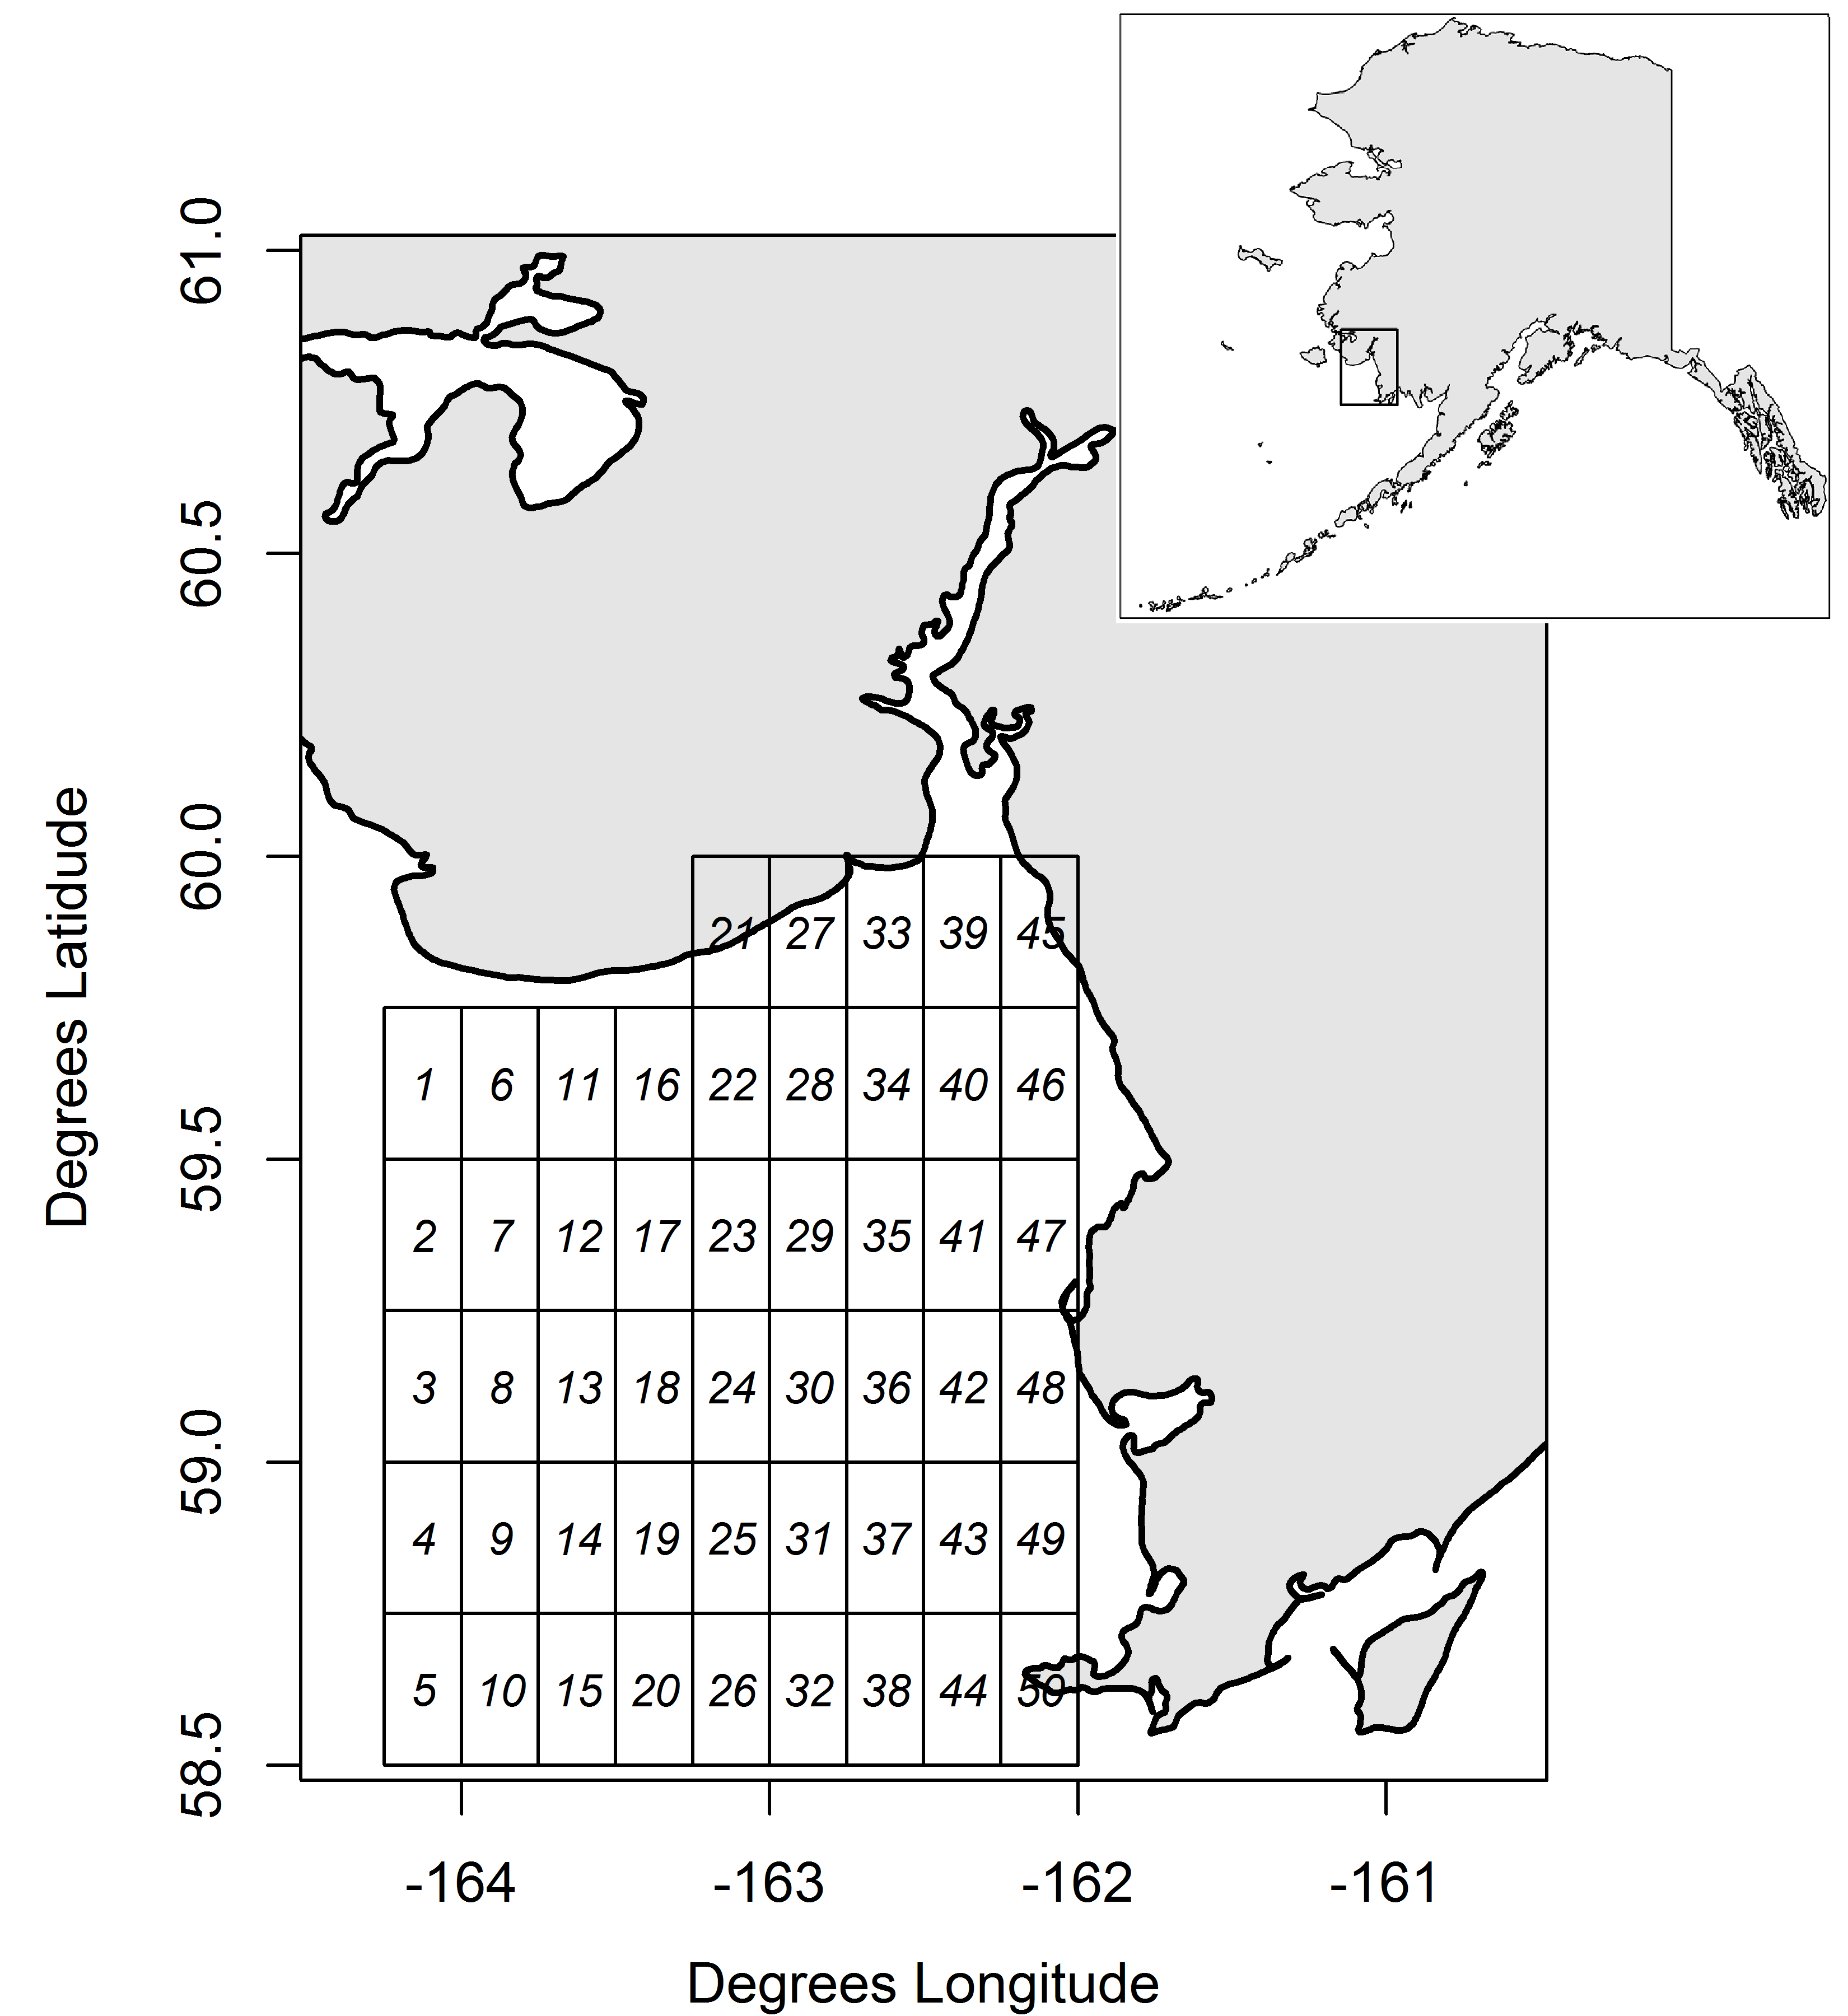
\includegraphics{img/Ch2/map.png}
  \caption{Map of Kuskokwim Bay where Chinook salmon likely stage for transition to freshwater. Shows grid cells from which daily SST values were used. Daily SIC values came from the same grid cells, though excluding grid cell 45 below due to missing values.}
  \label{fig:ch2-map}
\end{figure}

\clearpage

\begin{figure}
  \centering
  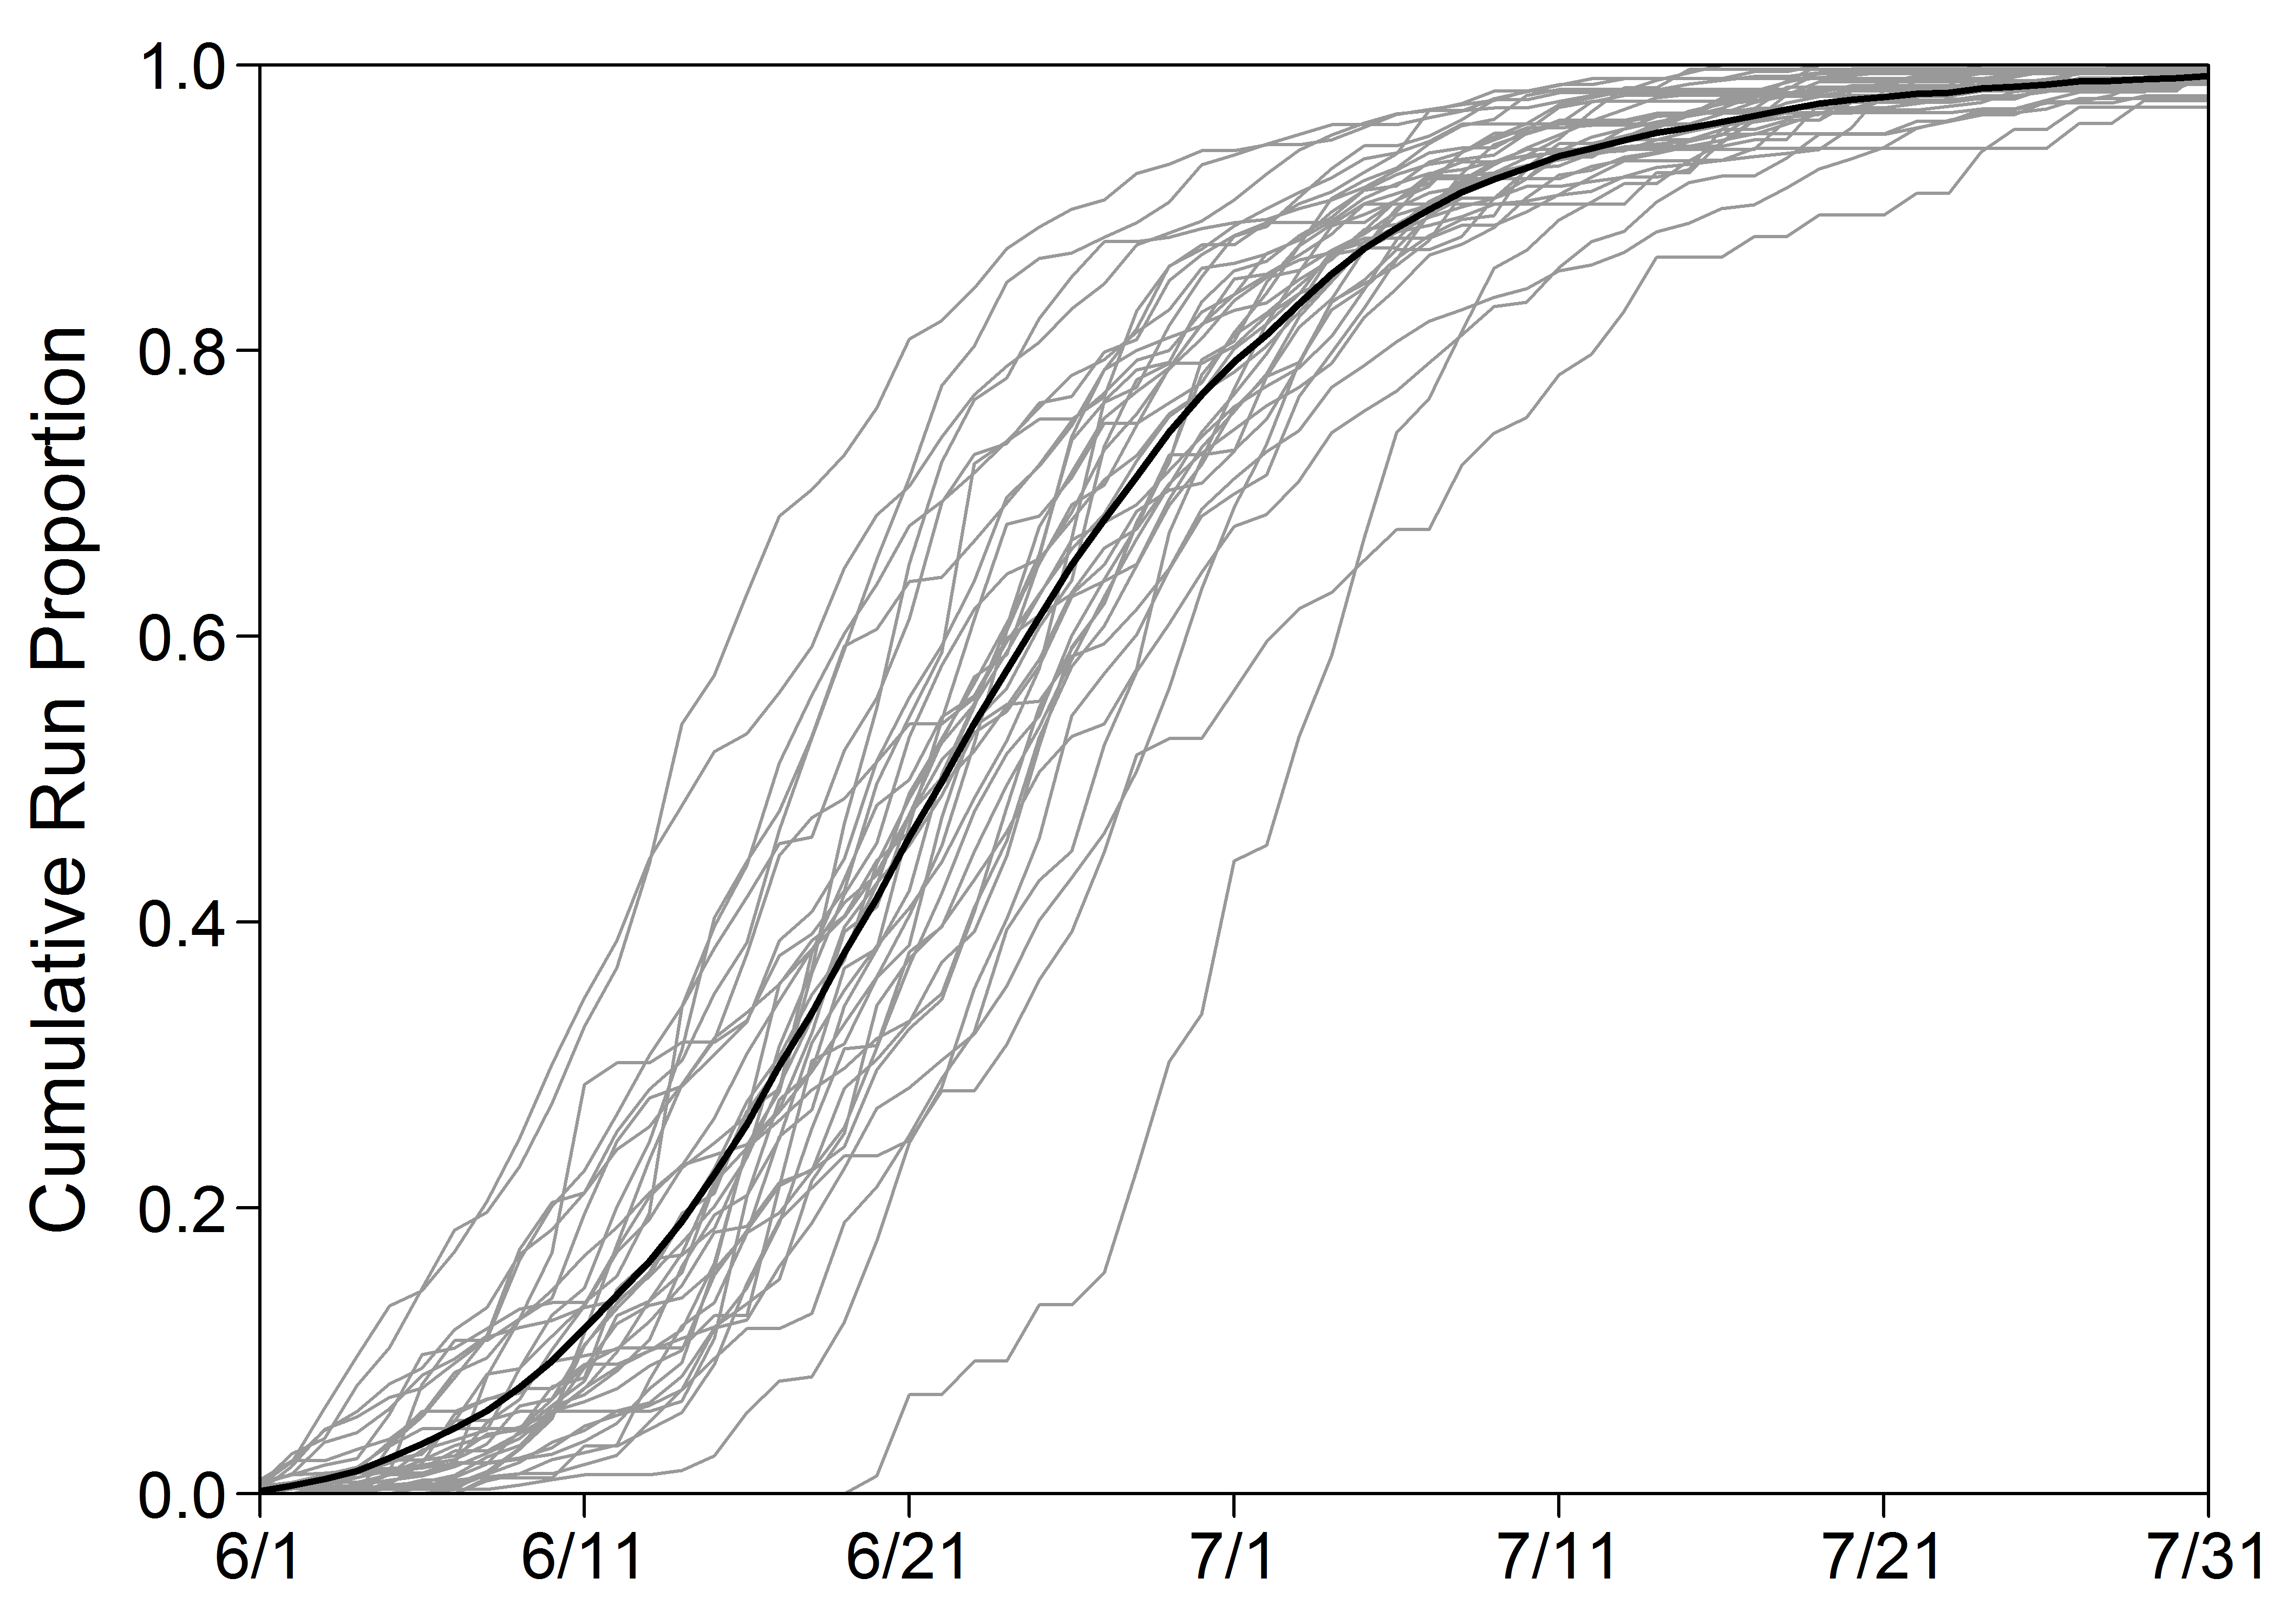
\includegraphics{img/Ch2/p-ccpue.png}
  \caption{Shape and variability of run timing patterns of the Kuskokwim River Chinook salmon stock as sampled by the Bethel Test Fishery, 1984 -- 2018. Each grey curve represents a year standardized by the total end-of-season cumulative CPUE and the black line represents the average value across years on each day of the season.}
  \label{fig:p-ccpue}
\end{figure}

\clearpage

\begin{figure}
  \centering
  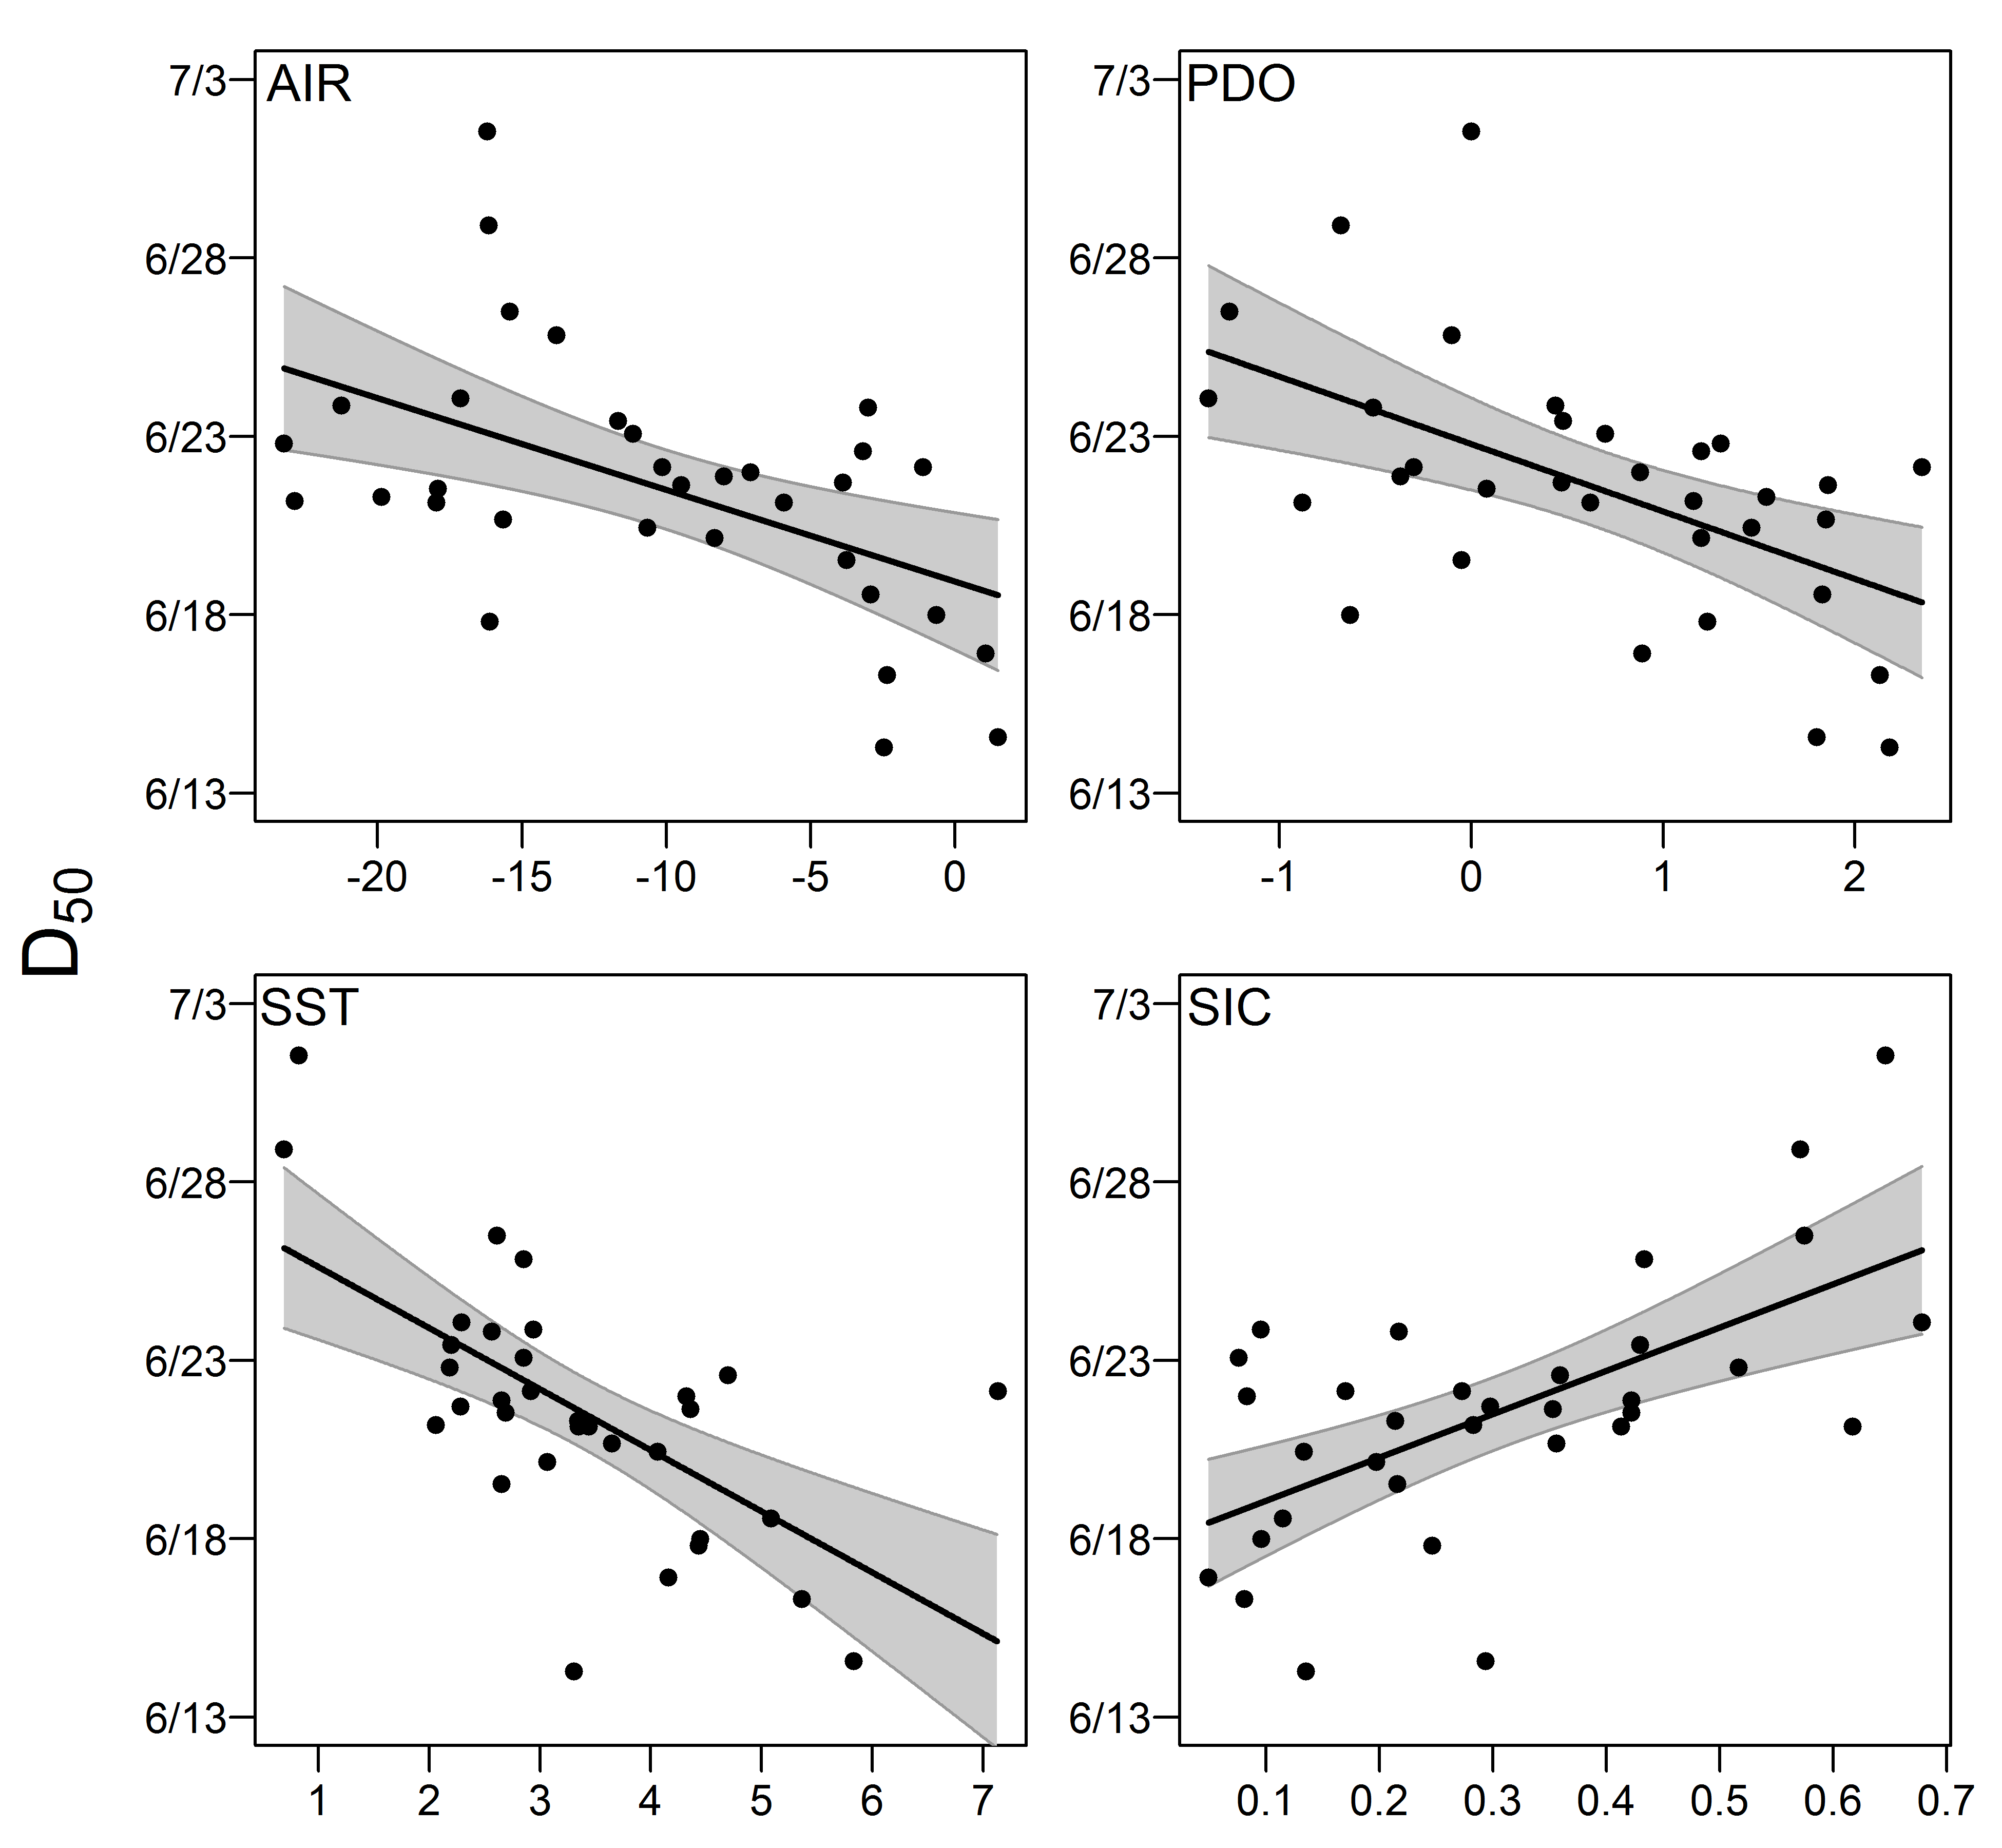
\includegraphics{img/Ch2/relationships.png}
  \caption{Relationships between the four single environmental variables and run timing $\left(D_{50}\right)$ using data from optimal climate windows when 2018 was added to the training data. For illustration purposes only, gridded variables SST and SIC were combined by weighted averaging where the weight of each grid cell was assigned the $\text{AIC}_{\text{c}}$ weight of that grid cell when grid cell-specific models were fit. Grey bands are 95$\%$ confidence intervals on the least squares line.}
  \label{fig:relationships}
\end{figure}

\clearpage

\begin{figure}
  \centering
  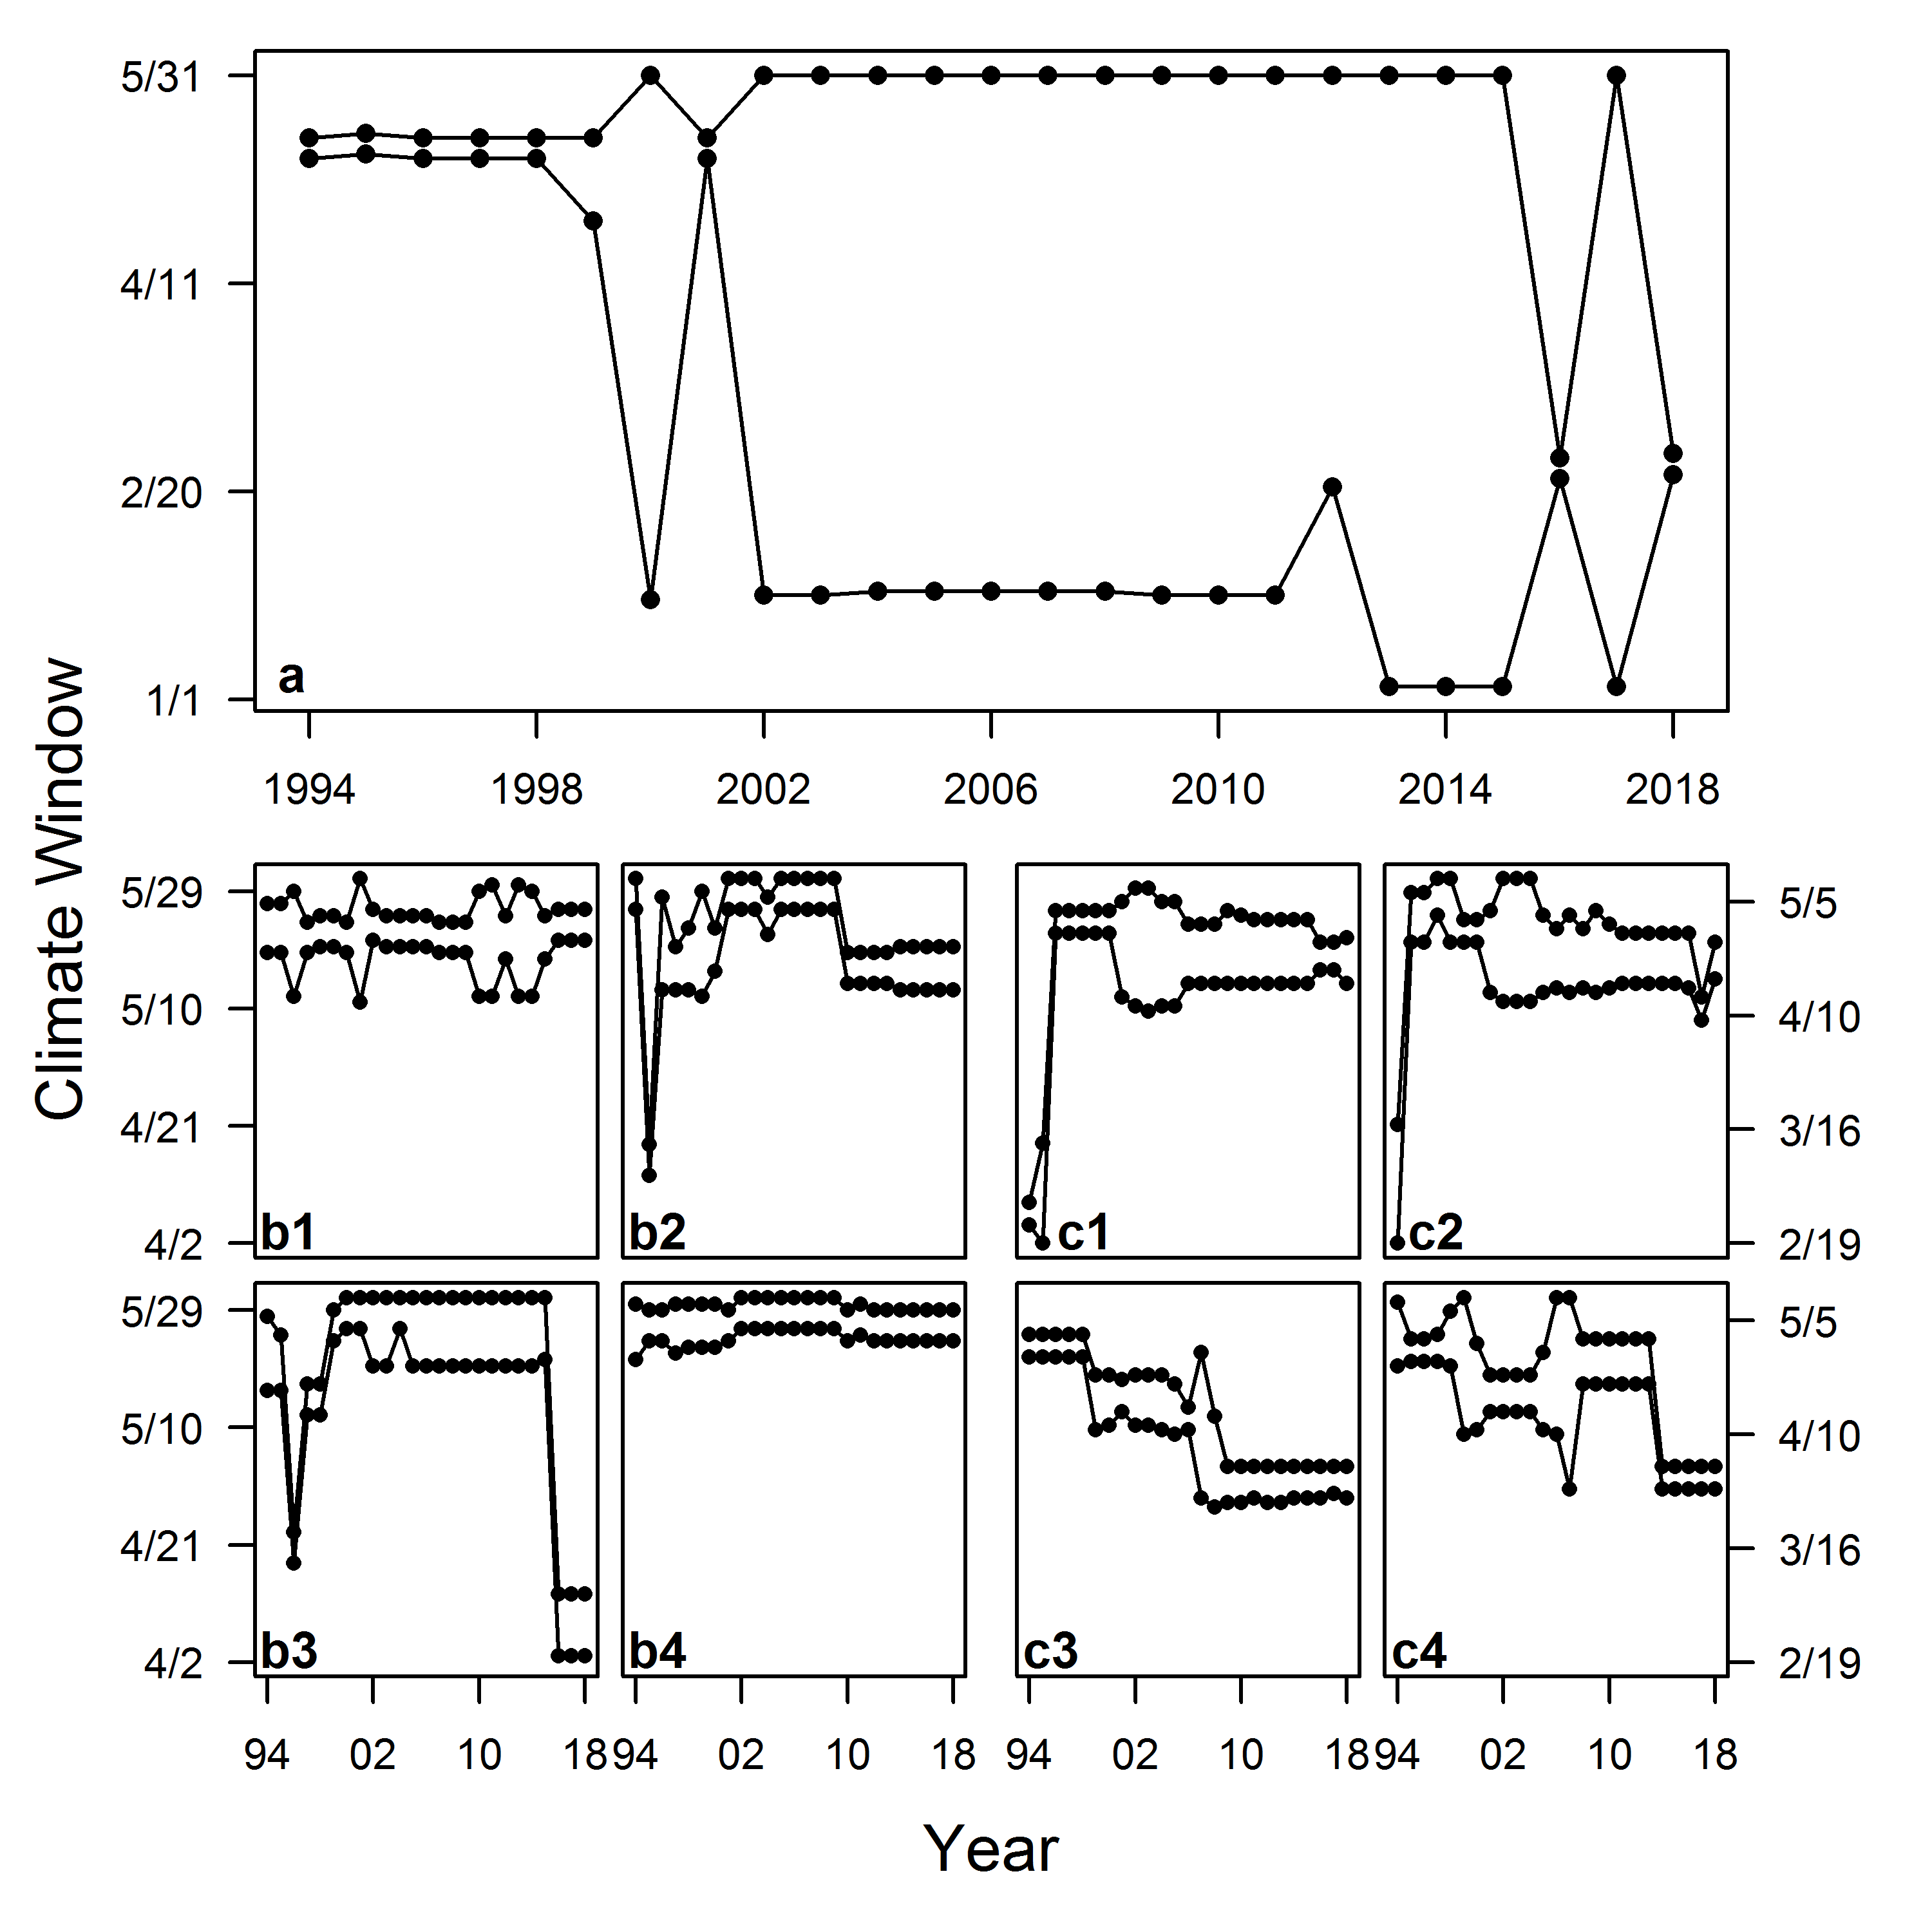
\includegraphics{img/Ch2/window-changes.png}
  \caption{Changes in selected climate windows as training data were added in the retrospective forecasting analysis. Bottom and top lines show the first and last day of the selected climate window, respectively, as more years were added. The year axis corresponds to the selected window after including environmental and run timing data from that year in the training data. E.g., the windows shown for 2017 were used to produce the forecast for 2018. Panel (a) is Bethel air temperature, panels b1-b4 are SST windows for four sample grid cells and panels c1-c4 are SIC windows for the same four sample grid cells. Sample grid cells from Figure \ref{fig:ch2-map} shown for SST and SIC are as follows: grid cell 8 (b1, c1), grid cell 44 (b2, c2), grid cell 12 (b3, c3), and grid cell 48 (b4, c4). Selected windows for PDO are not shown because the single month of May was selected in all years.}
  \label{fig:window-changes}
\end{figure}

\clearpage

\begin{figure}
  \centering
  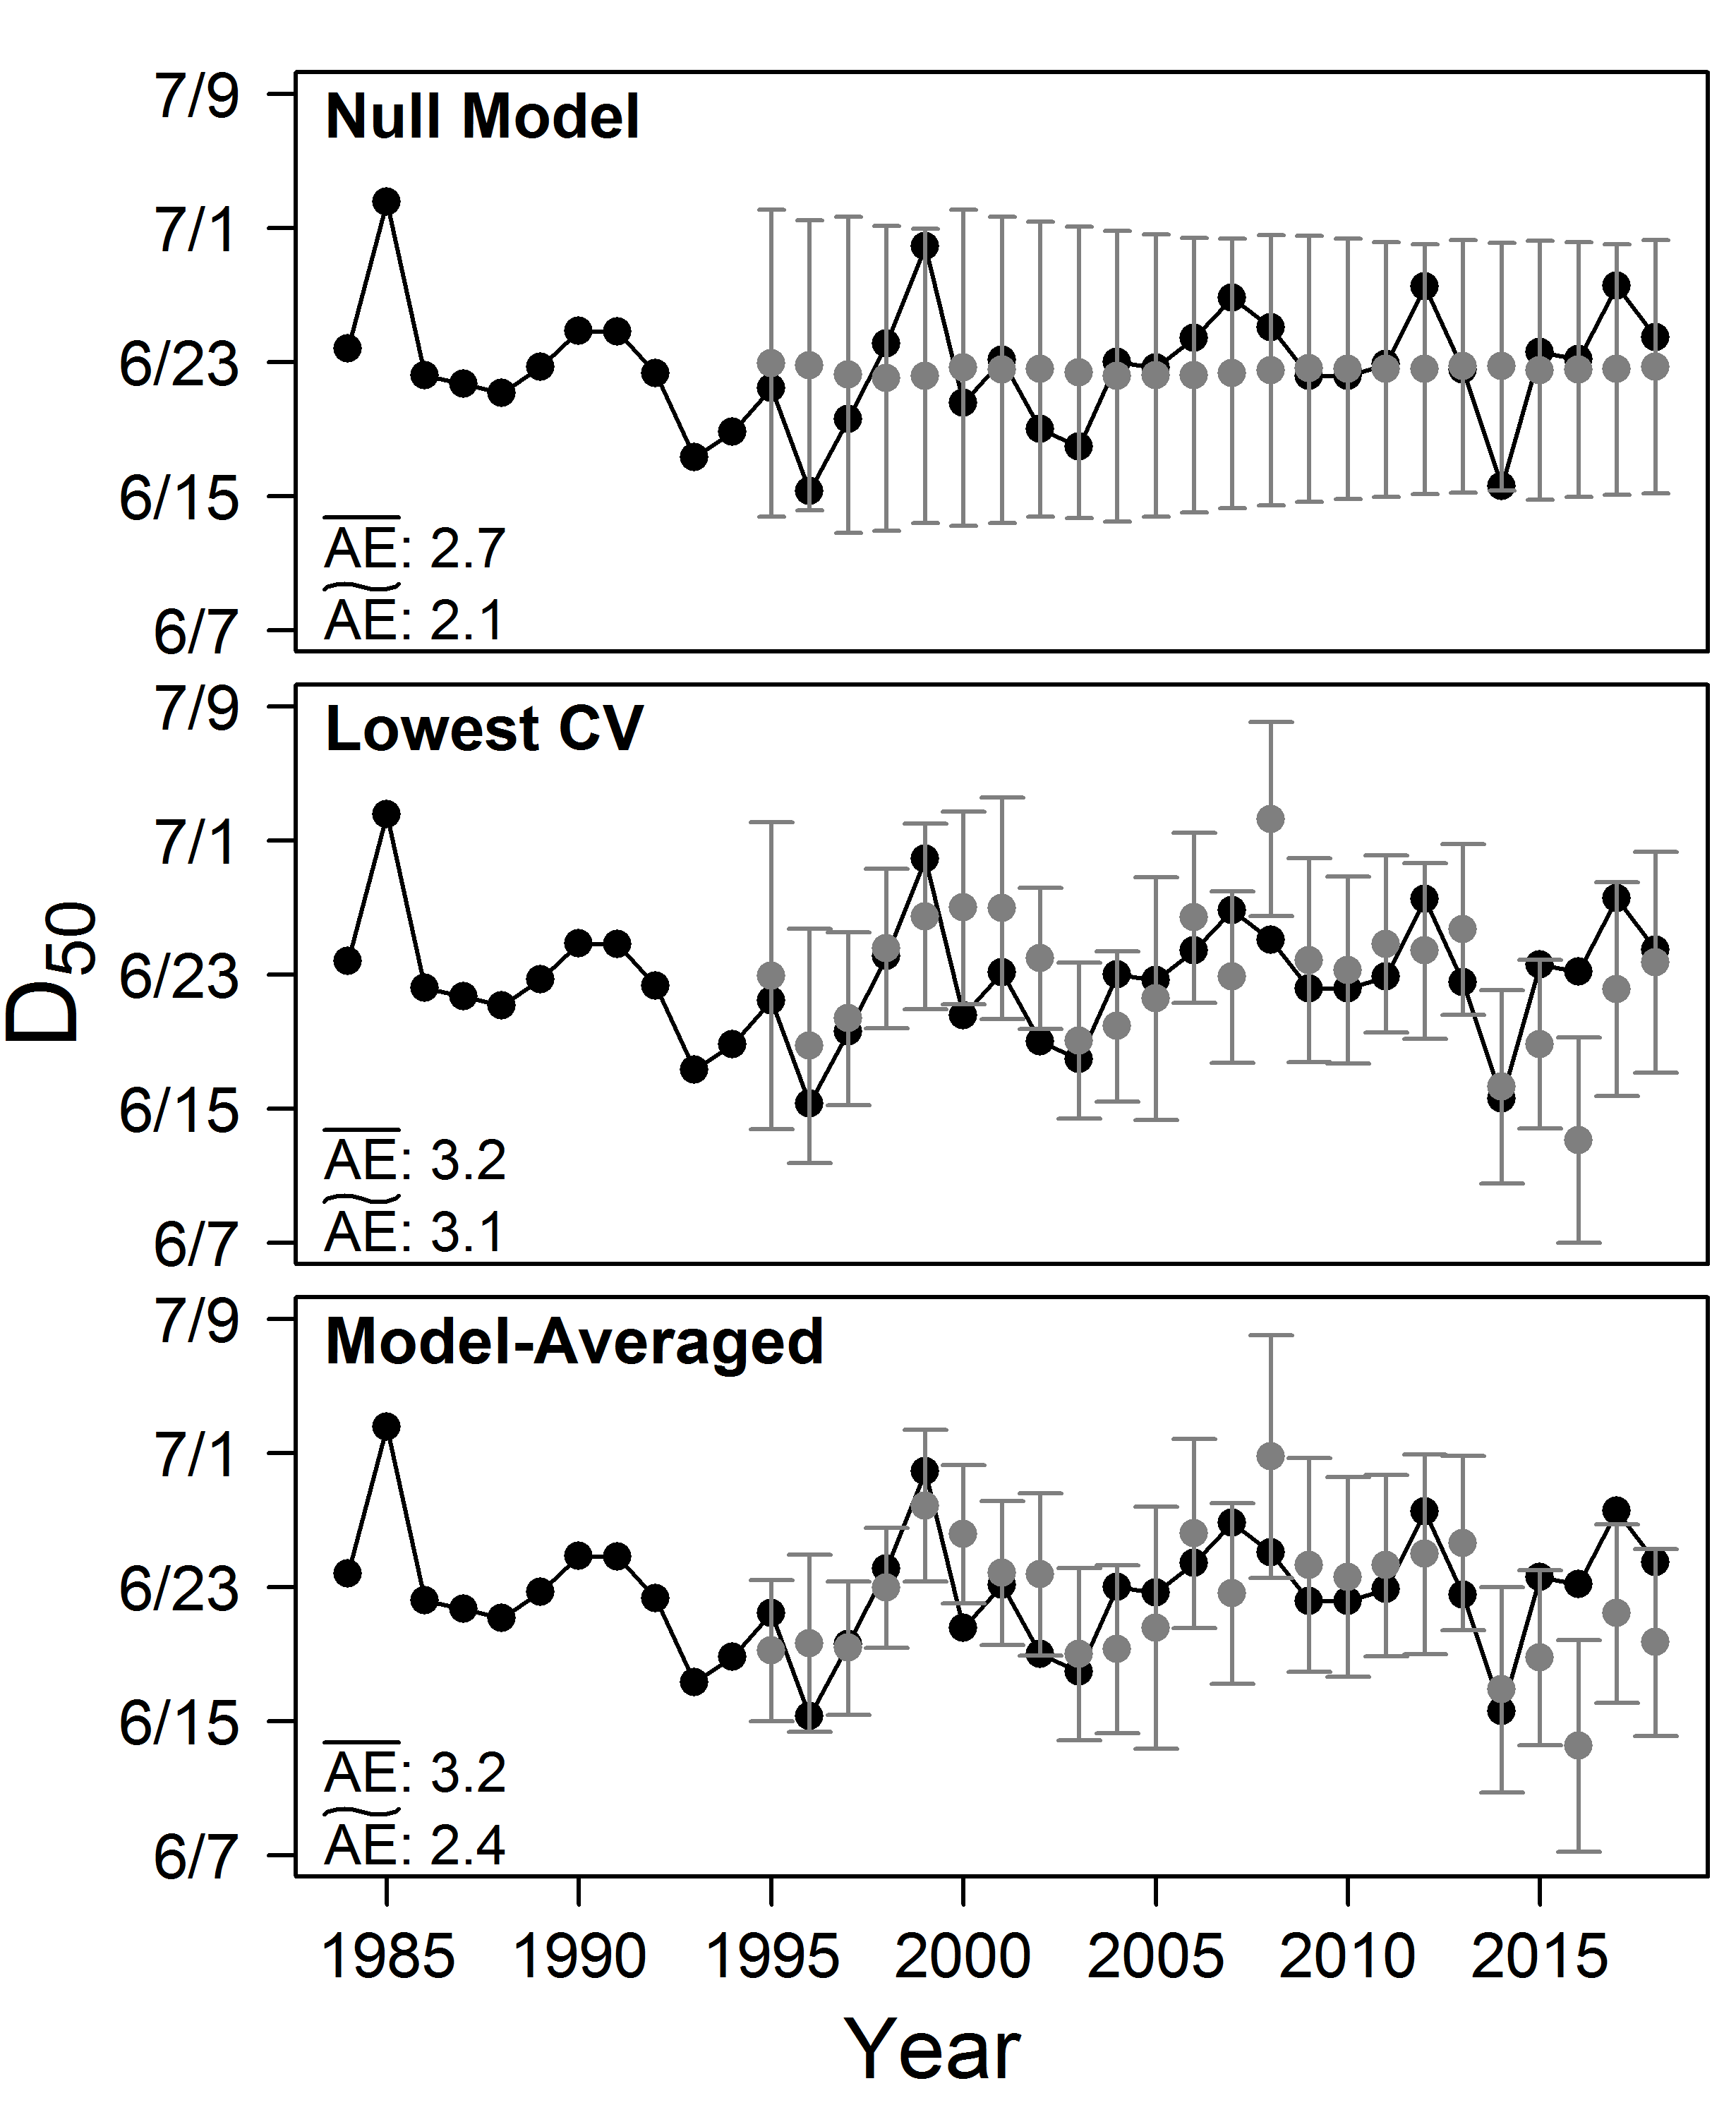
\includegraphics{img/Ch2/forecasts.png}
  \caption{Produced forecasts under the three approaches. Black points/lines are the time series of $D_{50}$ detected by the BTF. Grey points are out-of-sample forecasts with 95$\%$ prediction intervals shown as error bars. $\overline{\text{AE}}$ and $\widetilde{\text{AE}}$ are the mean and median absolute forecast errors from 1995 to 2018, respectively.}
  \label{fig:forecasts}
\end{figure}

\clearpage

\begin{figure}
  \centering
  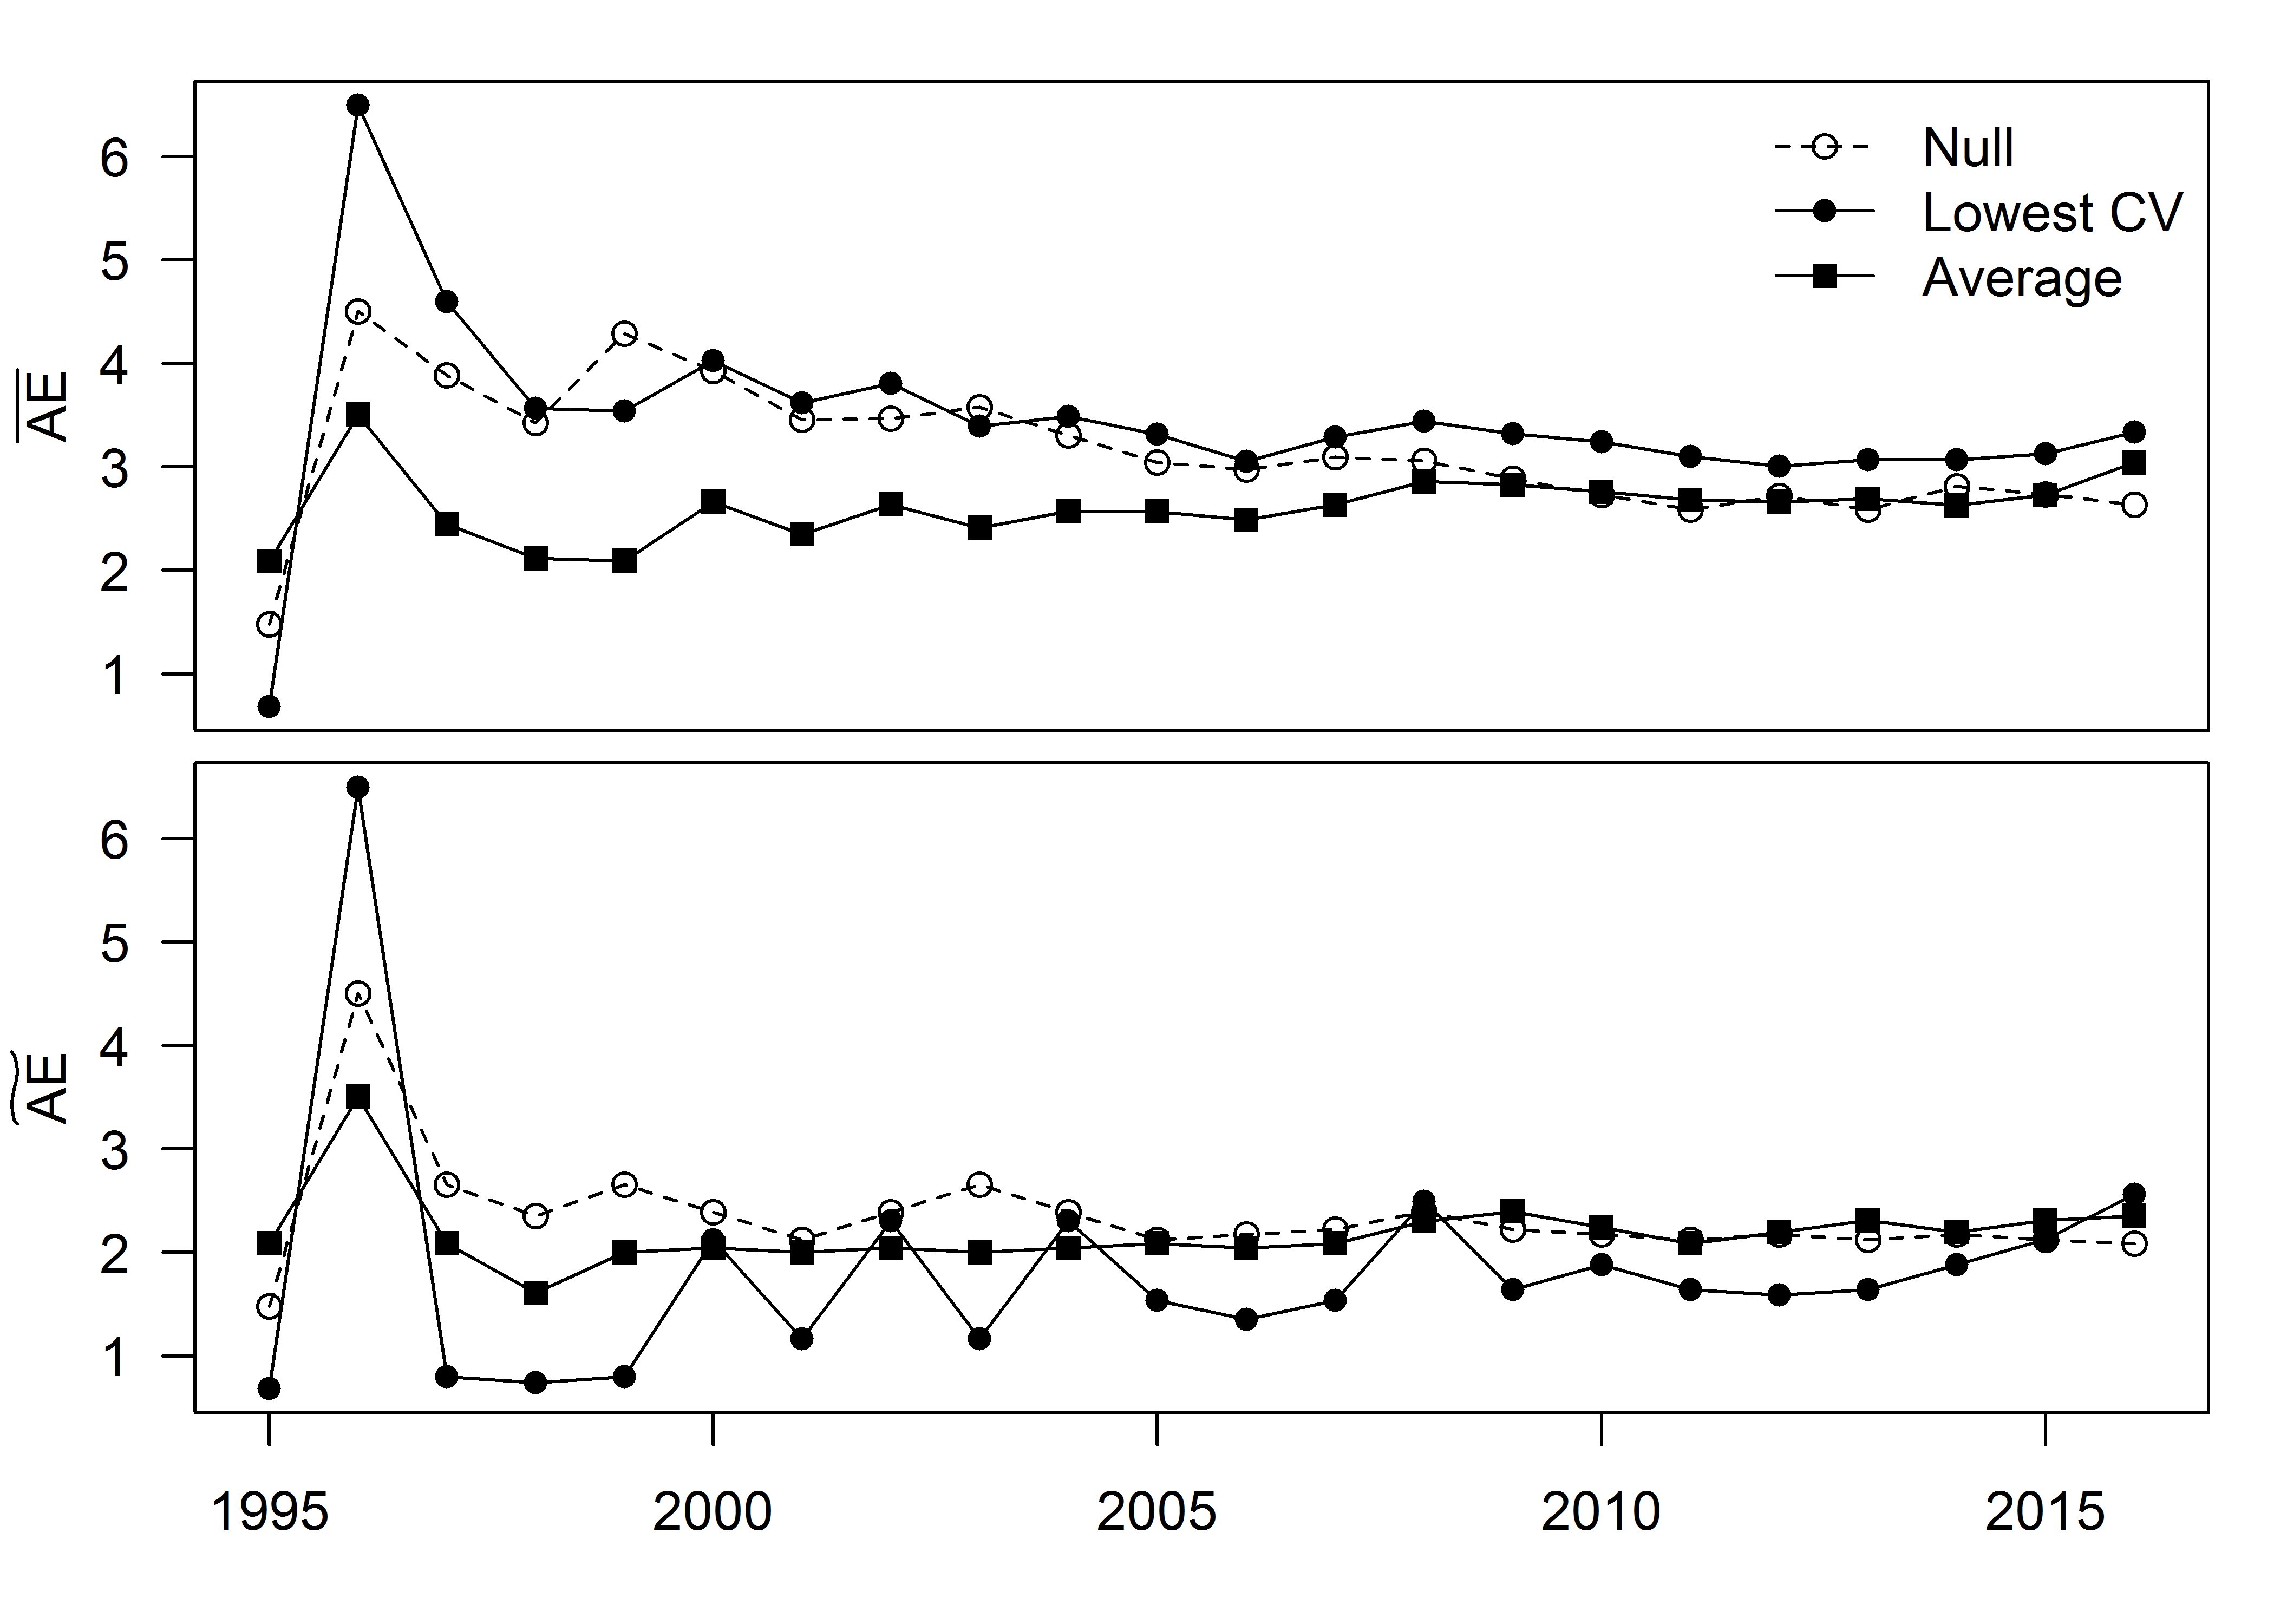
\includegraphics{img/Ch2/ae-changes.png}
  \caption{Evolution of $\overline{\text{AE}}$ (mean) and  $\overline{\text{AE}}$ (median) absolute forecast error under the three investigated forecasting approaches. Each point is the average of absolute errors of all years before and including the corresponding year on the $x$-axis, starting in 1995.}
  \label{fig:ae-changes}
\end{figure}

\clearpage

\begin{figure}
  \centering
  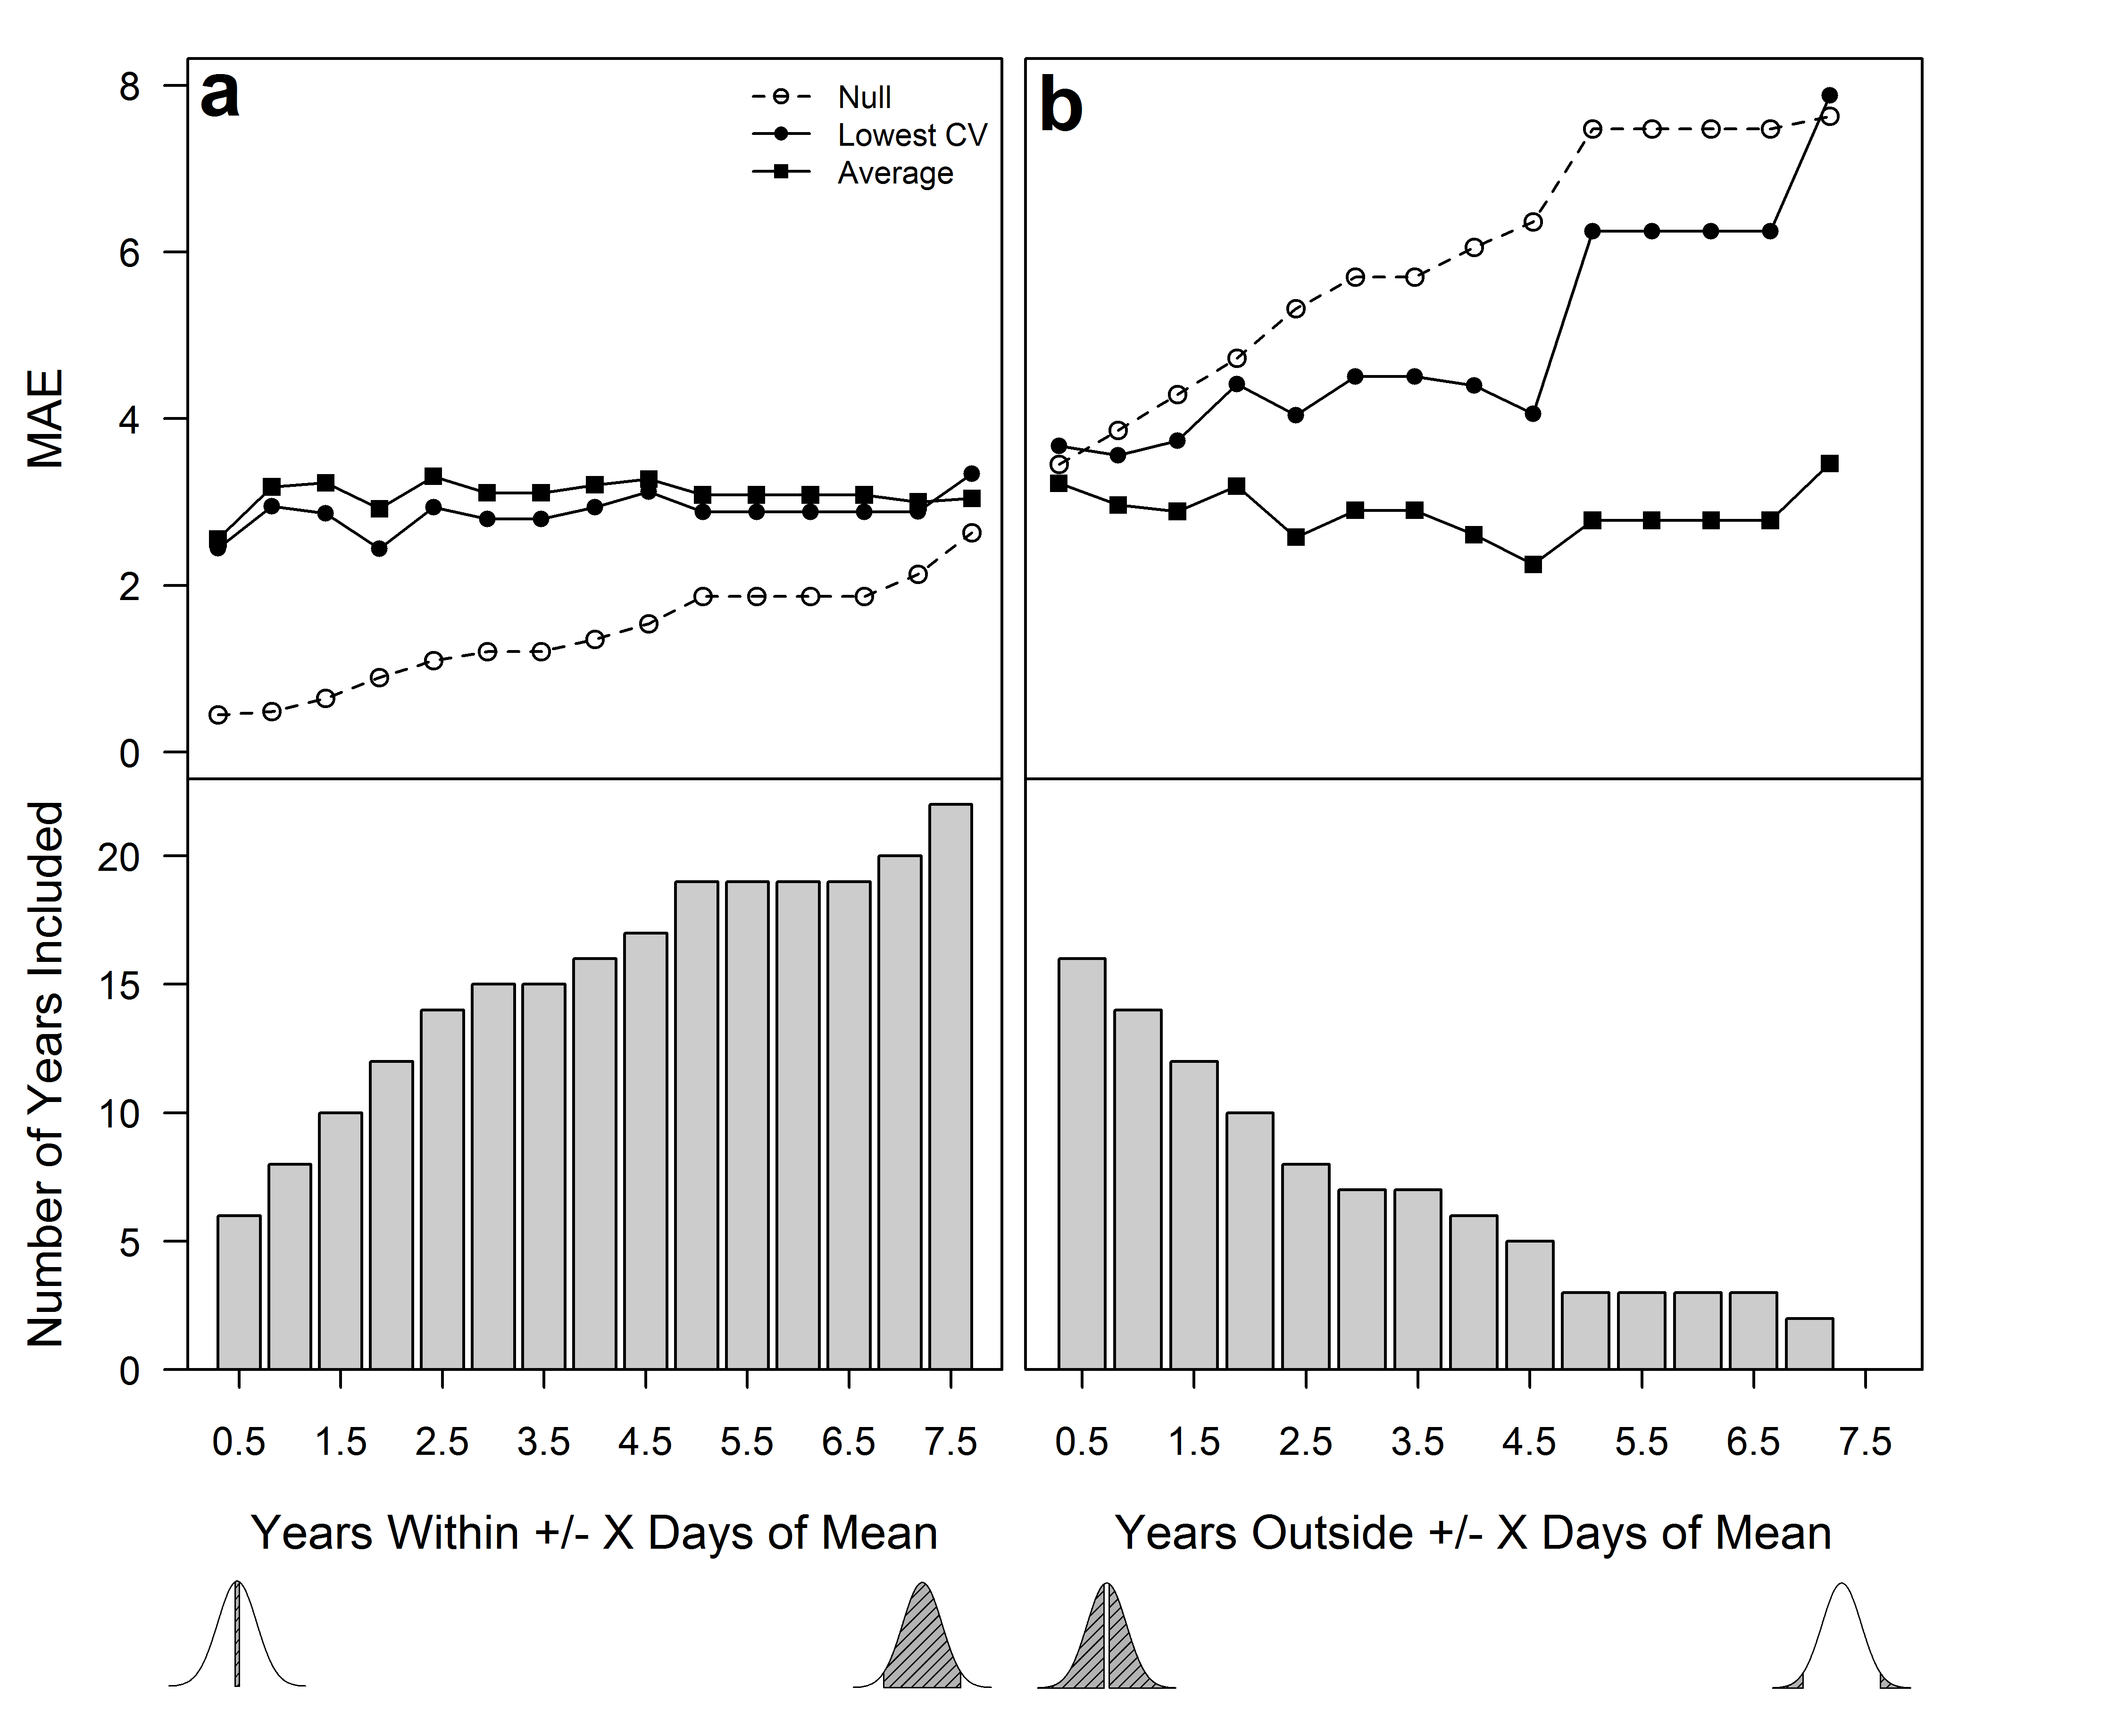
\includegraphics{img/Ch2/mae-subsets.png}
  \caption{$\overline{\text{AE}}$ under three forecast approaches calculated by either (a) including years with a $D_{50}$ value within $\pm x$  days of the all-year average or (b) including years with a $D_{50}$ value outside $\pm x$ days of average, where $x$ is the number of days indicated on the $x$-axis. Bottom panels show the number of observed years in which the appropriate $\pm x$ days criterion was met. Shaded regions in the hypothetical distributions show the types of $D_{50}$ values that were included in the calculation of $\overline{\text{AE}}$. One point that may enrich inference from this figure (and is shown in the shaded normal distributions) is that panel (a) becomes more inclusive from left to right by adding years that are more dissimilar to the average in the calculation of $\overline{\text{AE}}$ whereas panel (b) becomes more exclusive from left to right by removing years that are similar to the average.}
  \label{fig:mae-subsets}
\end{figure}

\clearpage

\begin{figure}
  \centering
  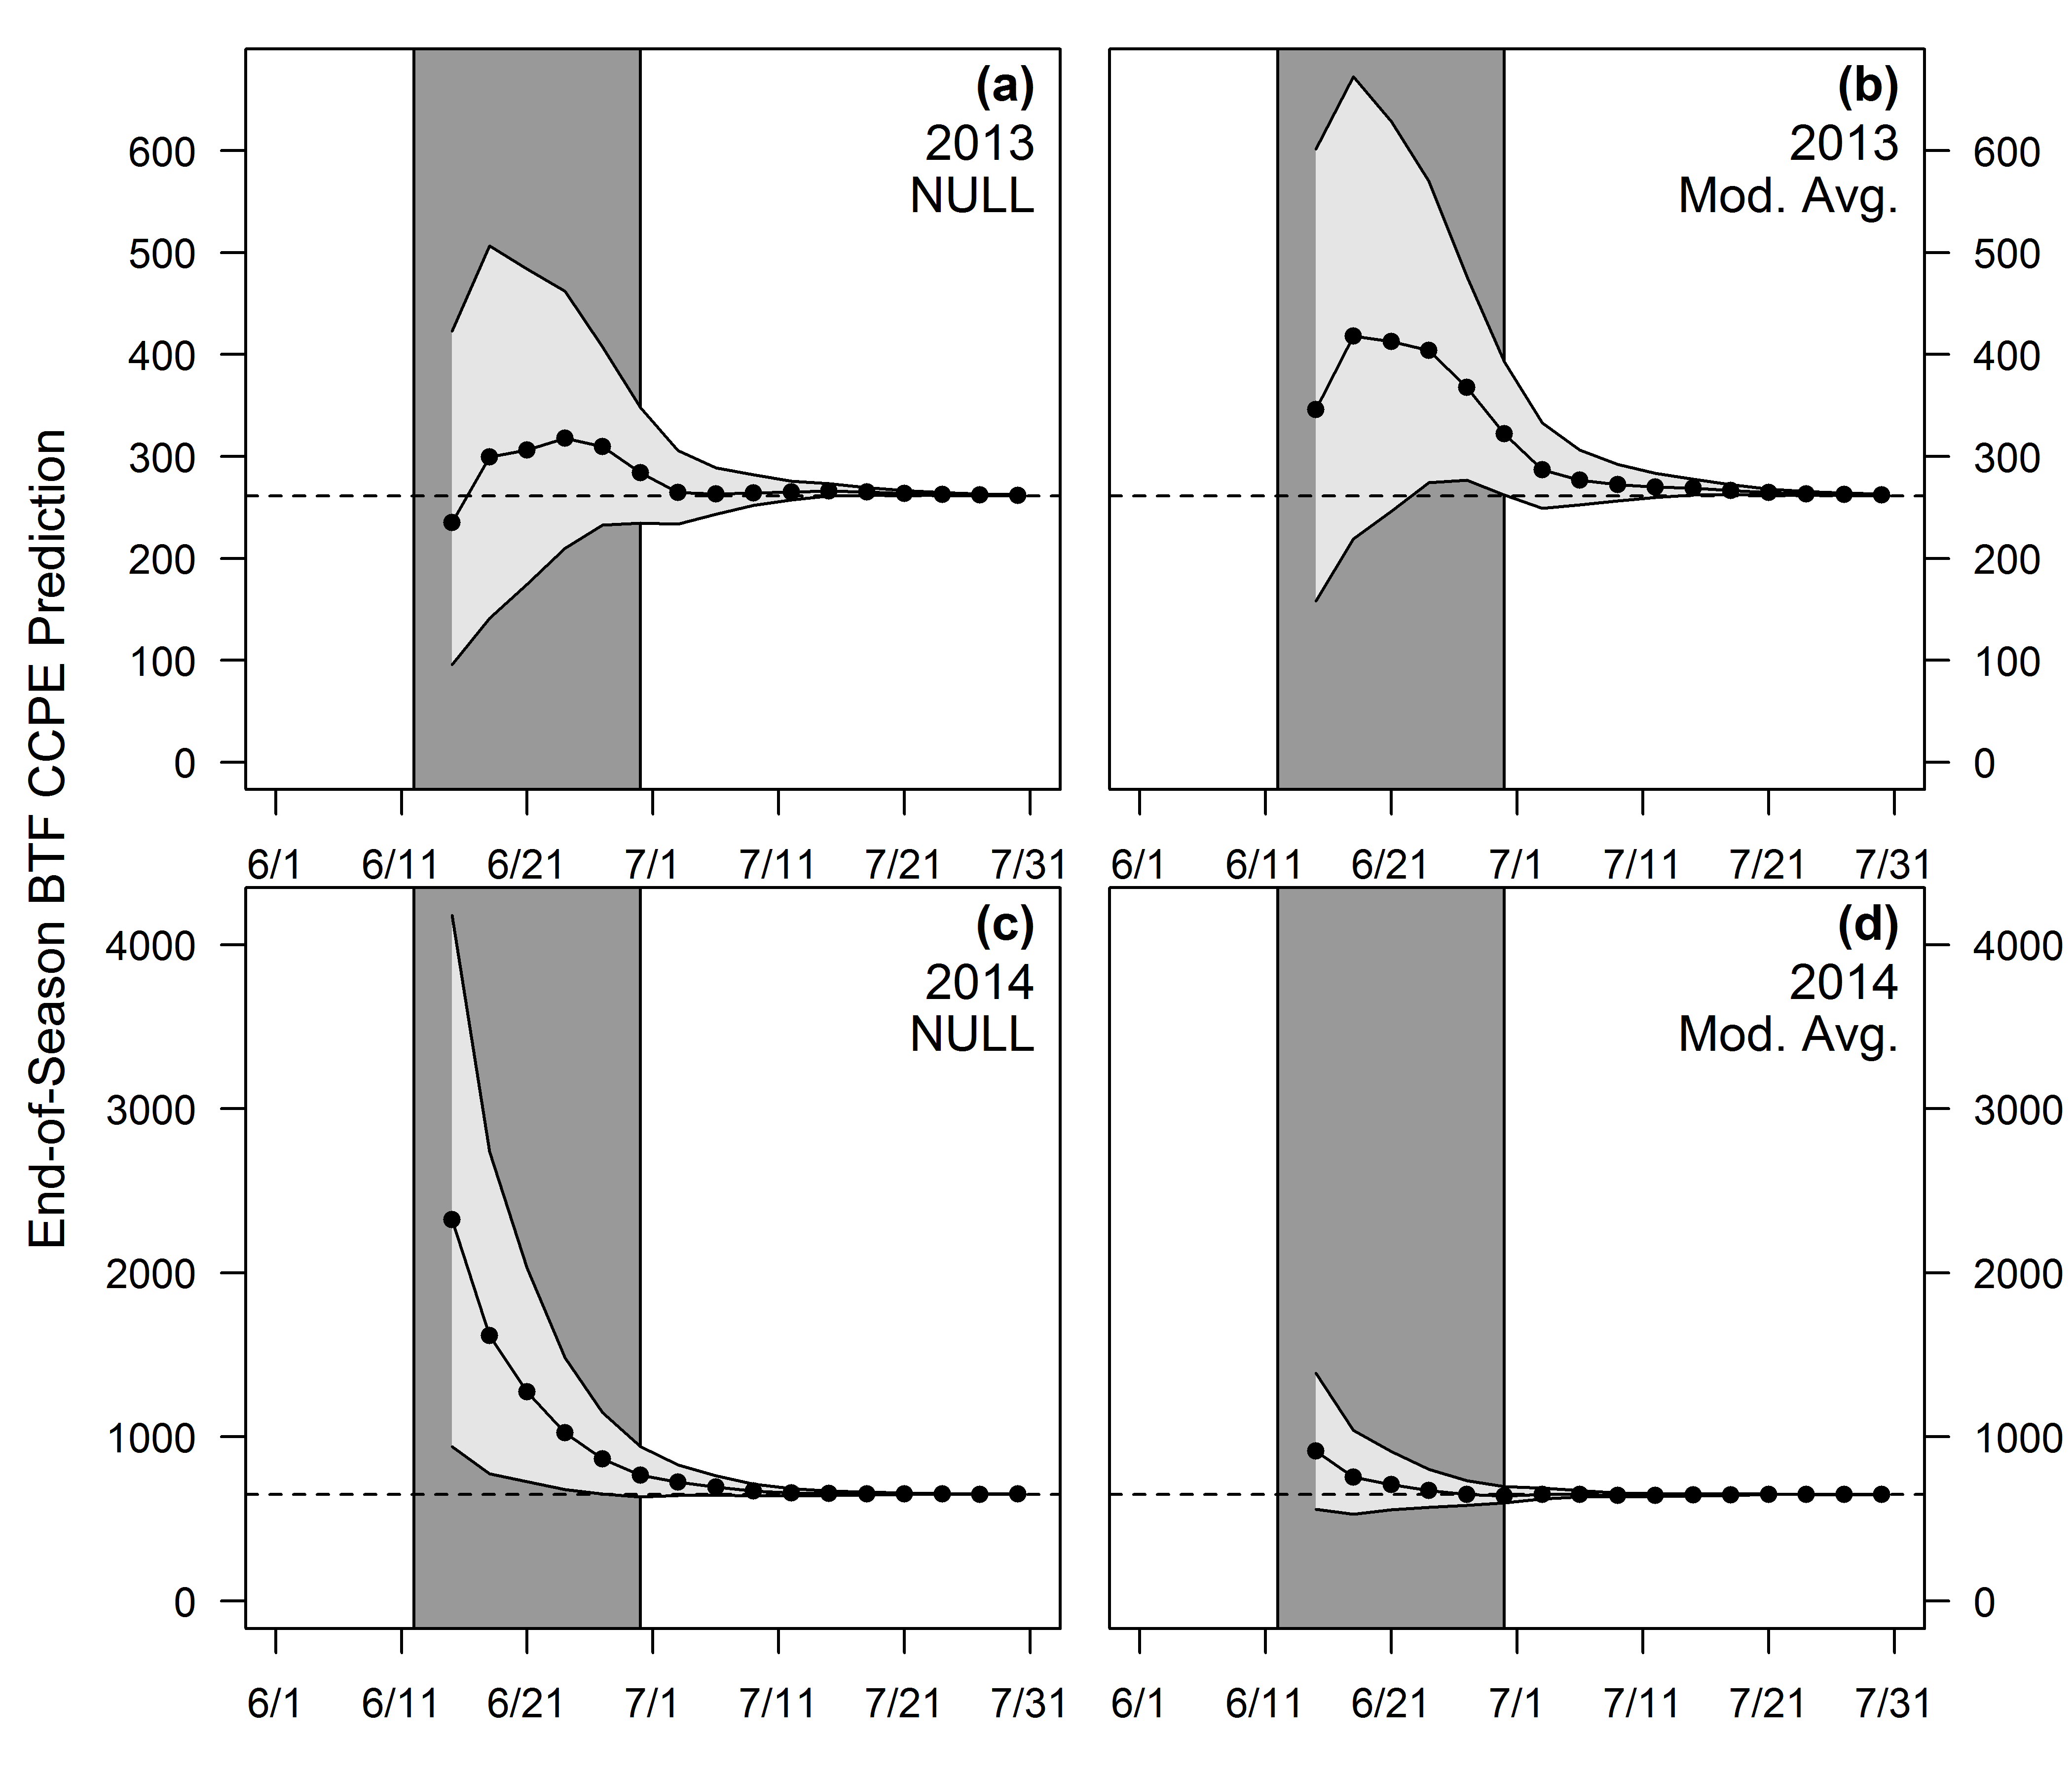
\includegraphics{img/Ch2/eos-preds.png}
  \caption{In-season predictions of end of season cumulative BTF CPUE under the model-averaged forecast using environmental variables and the forecast under the null model in 2013 and 2014. Intended to illustrate cases in which a manager would benefit from having access to the model-averaged run timing forecast model using environmental variables (2014) and when the null model would have performed better (2013). Horizontal lines are the true end of season cumulative BTF CPUE, dark grey regions are 50$\%$ confidence intervals, and light grey regions are 95$\%$ confidence intervals. Grey vertical lines indicate the period when key harvest decisions are made.}
  \label{fig:eos-preds}
\end{figure}

\begin{figure}
  \centering
  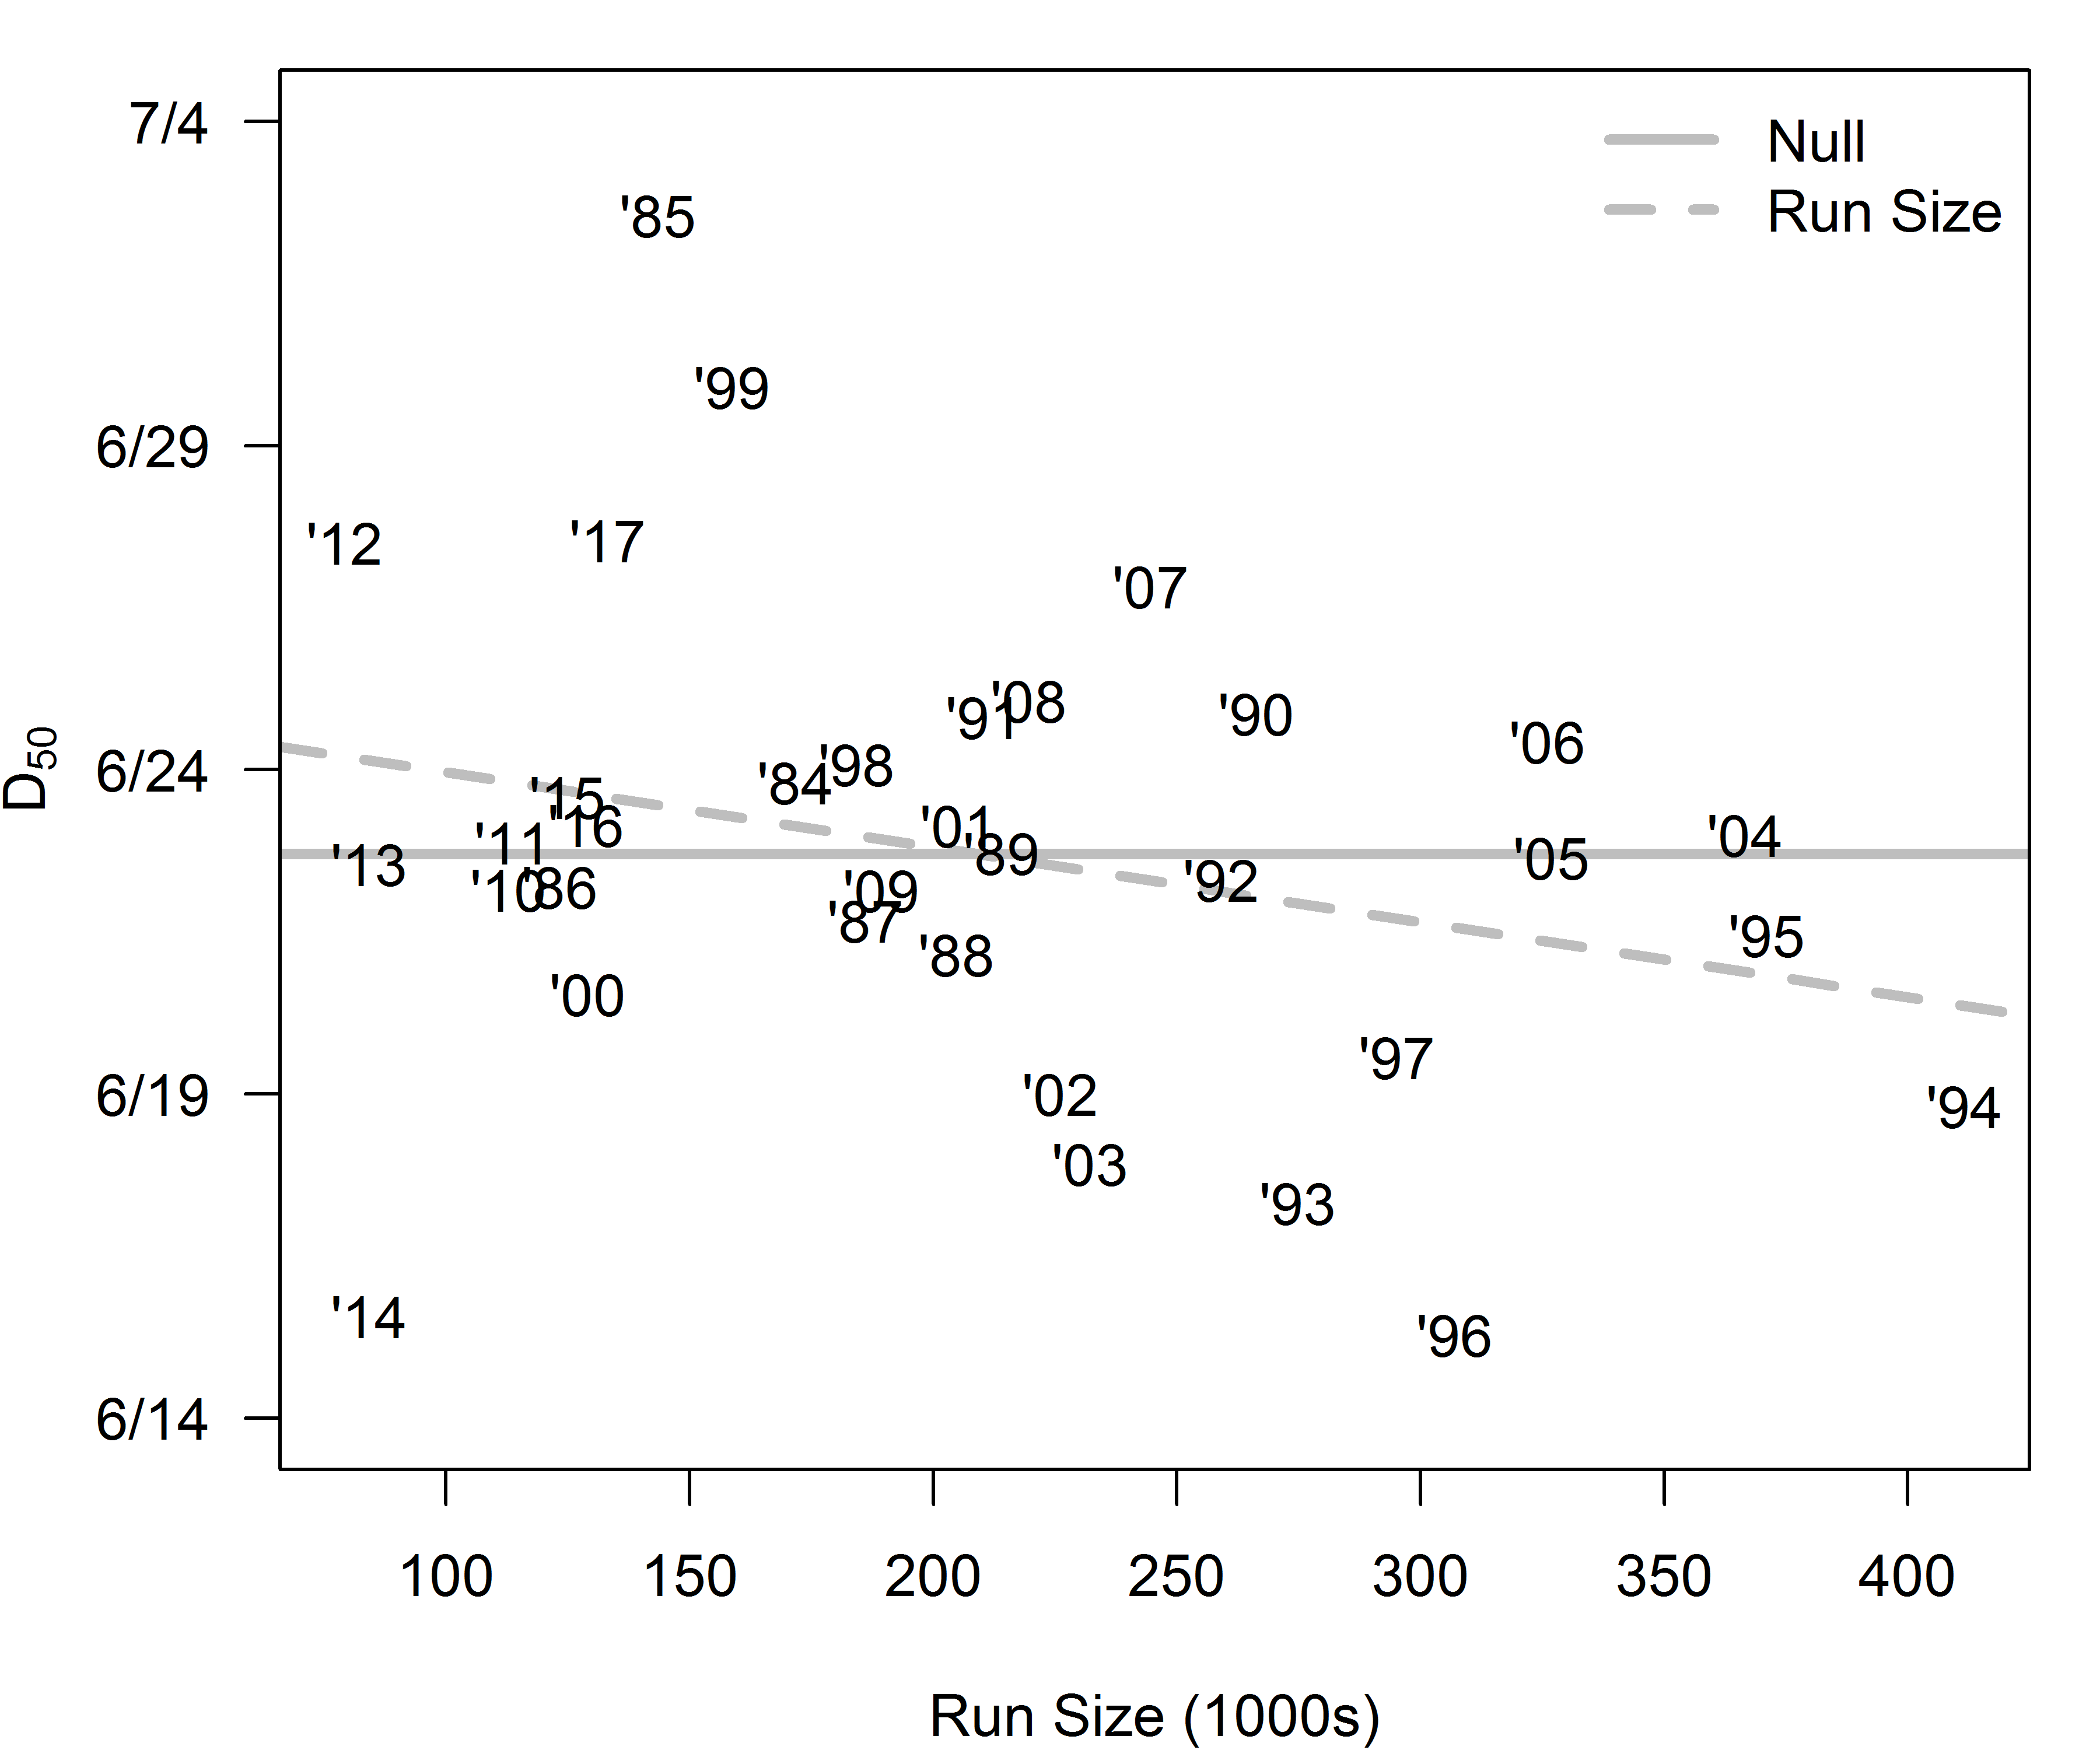
\includegraphics{img/Ch2/rt-n.png}
  \caption{Relationship between $D_{50}$ and run size for Kuskokwim River Chinook salmon with two fitted models shown: the null model (which assumed constant mean $D_{50}$) and the run size model (which assumed the mean $D_{50}$ changes as a function of run size). As described in the text, the effect of run size on run timing was very small and not significantly different than no effect. Additionally, knowledge of run size did not result in smaller average prediction errors of $D_{50}$ than not having this knowledge.}
  \label{fig:rt-n}
\end{figure}

\setlength{\parskip}{6pt plus 2pt minus 1pt}

\bibliography{cites-without-doi.bib,cites-with-doi.bib}


\end{document}
